% **************************************************
% Document Class Definition
% **************************************************
\documentclass[%
	paper=A4,					% paper size --> A4 is default in Germany
	twoside=true,				% onesite or twoside printing
	openright,					% doublepage cleaning ends up right side
	parskip=full,				% spacing value / method for paragraphs
	chapterprefix=true,			% prefix for chapter marks
	11pt,						% font size
	headings=normal,			% size of headings
	bibliography=totoc,			% include bib in toc
	listof=totoc,				% include listof entries in toc
	titlepage=on,				% own page for each title page
	captions=tableabove,		% display table captions above the float env
	draft=false,				% value for draft version
]{scrreprt}%

% **************************************************
% Debug LaTeX Information
% **************************************************
%\listfiles

% **************************************************
% Information and Commands for Reuse
% **************************************************
\newcommand{\ie}{\textit{i.e.,}\xspace}
\newcommand{\eg}{\textit{e.g.,}\xspace}
\newcommand{\etc}{\textit{etc.}\xspace}
\newcommand{\thesisTitle}{Automated extraction of augmented models for native and hybrid mobile applications in Android}
\newcommand{\thesisName}{Santiago Li\~{n}\'{a}n Romero}
\newcommand{\thesisSubject}{Thesis submitted to the Faculty of Engineering in
	partial fulfillment of the requirements
	for the degree of MSc. in Software Engineering}
\newcommand{\thesisDate}{December, 2018}
\newcommand{\thesisVersion}{Full draft - Prior Advisor review}

\newcommand{\thesisFirstReviewer}{Ph.D. Nicol\'{a}s Cardozo }
\newcommand{\thesisFirstReviewerUniversity}{\protect{Universidad de los Andes, Bogot\'{a}, Colombia}}
\newcommand{\thesisFirstReviewerDepartment}{Systems and Computing Engineering Department}

\newcommand{\thesisSecondReviewer}{Ph.D. Gabriele Bavota}
\newcommand{\thesisSecondReviewerUniversity}{\protect{Universit\`{a} della Svizzera italiana (USI), Lugano}}
\newcommand{\thesisSecondReviewerDepartment}{Faculty of Informatics }

\newcommand{\thesisFirstSupervisor}{Ph.D. Mario Linares V\'{a}squez}

\newcommand{\thesisUniversity}{\protect{Universidad de los Andes}}
\newcommand{\thesisUniversityDepartment}{Systems and Computing Engineering Department}
\newcommand{\thesisUniversityInstitute}{Faculty of Engineering}
\newcommand{\thesisUniversityGroup}{The Software Design Lab}
\newcommand{\thesisUniversityCity}{Bogot\'{a}, Colombia}
\newcommand{\thesisUniversityStreetAddress}{Cra 1 \# 18A - 12}
\newcommand{\thesisUniversityPostalCode}{111711}



% **************************************************
% Load and Configure Packages
% **************************************************
\usepackage[utf8]{inputenc}		% defines file's character encoding
\usepackage[english]{babel} % babel system, adjust the language of the content
\usepackage[					% clean thesis style
	figuresep=colon,%
	sansserif=false,%
	hangfigurecaption=false,%
	hangsection=true,%
	hangsubsection=true,%
	colorize=full,%
	colortheme=bluemagenta,%
	bibsys=bibtex,%
	bibfile=bib-refs,%
	bibstyle=numeric,%
]{cleanthesis}
\usepackage[linesnumbered]{algorithm2e}
\usepackage{adjustbox}
\usepackage{listings,color}
\usepackage{amsfonts}
\usepackage{tcolorbox}
\usepackage{amssymb}
\usepackage{ifthen}
\lstset{
	language=xml,
	tabsize=2,
	%frame=lines,
	frame=shadowbox,
	rulesepcolor=\color{gray},
	xleftmargin=18pt,
	framexleftmargin=15pt,
	keywordstyle=\color{blue},
	commentstyle=\color{OliveGreen},
	stringstyle=\color[rgb]{0,0.43,0.72},
	numbers=left,
	numberstyle=\tiny,
	numbersep=4pt,
	breaklines=true,
	showstringspaces=false,
	basicstyle=\ttfamily\scriptsize,
	columns=fullflexible,
	emph={node,name,price},emphstyle={\color{magenta}}}

\colorlet{punct}{red!60!black}
\definecolor{background}{HTML}{EEEEEE}
\definecolor{delim}{RGB}{20,105,176}
\colorlet{numb}{magenta!60!black}
\lstdefinelanguage{json}{
	basicstyle=\ttfamily\scriptsize,
	numbers=left,
	numberstyle=\scriptsize,
	stepnumber=1,
	numbersep=8pt,
	showstringspaces=false,
	breaklines=true,
	frame=shadowbox,
	literate=
	*{0}{{{\color{numb}0}}}{1}
	{1}{{{\color{numb}1}}}{1}
	{2}{{{\color{numb}2}}}{1}
	{3}{{{\color{numb}3}}}{1}
	{4}{{{\color{numb}4}}}{1}
	{5}{{{\color{numb}5}}}{1}
	{6}{{{\color{numb}6}}}{1}
	{7}{{{\color{numb}7}}}{1}
	{8}{{{\color{numb}8}}}{1}
	{9}{{{\color{numb}9}}}{1}
	{:}{{{\color{punct}{:}}}}{1}
	{,}{{{\color{punct}{,}}}}{1}
	{\{}{{{\color{delim}{\{}}}}{1}
	{\}}{{{\color{delim}{\}}}}}{1}
	{[}{{{\color{delim}{[}}}}{1}
	{]}{{{\color{delim}{]}}}}{1},
}

\lstloadlanguages{xml}
\renewcommand{\lstlistingname}{Code example}% Listing -> Algorithm
\renewcommand{\lstlistlistingname}{List of \lstlistingname s}


\hypersetup{					% setup the hyperref-package options
	pdftitle={\thesisTitle},	% 	- title (PDF meta)
	pdfsubject={\thesisSubject},% 	- subject (PDF meta)
	pdfauthor={\thesisName},	% 	- author (PDF meta)
	plainpages=false,			% 	-
	colorlinks=false,			% 	- colorize links?
	pdfborder={0 0 0},			% 	-
	breaklinks=true,			% 	- allow line break inside links
	bookmarksnumbered=true,		%
	bookmarksopen=true			%
}

\newcommand{\nb}[2]{
	\fbox{\bfseries\sffamily\scriptsize#1}
	{\small$\blacktriangleright$\textit{#2}$\blacktriangleleft$}}
\newcommand\MARIO[1]{\textcolor{red}{\nb{MARIO}{#1}}}
% **************************************************
% Document CONTENT
% **************************************************
\begin{document}

% --------------------------
% rename document parts
% --------------------------
%\renewcaptionname{ngerman}{\figurename}{Abb.}
%\renewcaptionname{ngerman}{\tablename}{Tab.}
\renewcaptionname{english}{\figurename}{Fig.}
\renewcaptionname{english}{\tablename}{Tab.}

% --------------------------
% Front matter
% --------------------------
\pagenumbering{roman}			% roman page numbing (invisible for empty page style)
\pagestyle{empty}				% no header or footers
% !TEX root = ../thesis-example.tex
%
% ------------------------------------  --> cover title page
\begin{titlepage}
	\pdfbookmark[0]{Cover}{Cover}
	\flushright
	\hfill
	\vfill
	{\LARGE\thesisTitle \par}
	\rule[5pt]{\textwidth}{.4pt} \par
	{\Large\thesisName}
	\vfill
	\textit{\large\thesisDate} \\
	Version: \thesisVersion
\end{titlepage}


% ------------------------------------  --> main title page
\begin{titlepage}
	\pdfbookmark[0]{Titlepage}{Titlepage}
	\tgherosfont
	\centering

	Bogotá, Colombia \\[4mm]
	
\includegraphics[width=6cm]{gfx/logo-uniandes} \\[2mm]
	\textsf{\thesisUniversityDepartment} \\
	\textsf{\thesisUniversityInstitute} \\
	\textsf{\thesisUniversityGroup} \\

	\vfill
	{\large \thesisSubject} \\[5mm]
	{\LARGE \color{ctcolortitle}\textbf{\thesisTitle} \\[10mm]}
	{\Large \thesisName} \\

	\vfill
		\begin{minipage}[t]{.27\textwidth}
		\raggedleft
		\textit{Asesor}
	\end{minipage}
	\hspace*{15pt}
	\begin{minipage}[t]{.65\textwidth}
		{\Large \thesisFirstSupervisor} \\
		{\small \thesisFirstReviewerDepartment} \\[-1mm]
		{\small \thesisFirstReviewerUniversity}
	\end{minipage} \\[5mm]

	\thesisDate \\

\end{titlepage}


% ------------------------------------  --> lower title back for single page layout
\hfill
\vfill
{
	\small
	\textbf{\thesisName} \\
	\textit{\thesisTitle} \\
	\thesisSubject, \thesisDate \\
	Asesor: \thesisFirstSupervisor\\[1.5em]
	\textbf{\thesisUniversity} \\
	\textit{\thesisUniversityGroup} \\
	\thesisUniversityInstitute \\
	\thesisUniversityDepartment \\
	\thesisUniversityStreetAddress \\
	\thesisUniversityPostalCode\ and \thesisUniversityCity
}
		% INCLUDE: all titlepages
\cleardoublepage

\pagestyle{plain}				% display just page numbers
% !TEX root = ../thesis-example.tex
%
\pdfbookmark[0]{Abstract}{Abstract}
\chapter*{Abstract}
\label{sec:abstract}
\vspace*{-10mm}
Mobile software development involves significant challenges to developers such as device fragmentation (\ie enormous hardware and software diversity), event-driven programming (\ie programming based on user interactions, sensor readings and other events where the program must react) and continuous evolving platforms (\ie fast changing mobile frameworks and technologies). This can lead programmers to error-prone code, because of the multiple combinations of external variables that must be taken into account in an app development process. Thus, testing is an underlying necessity in mobile applications to deliver high quality apps. However, defining tests suites for app development is a difficult task that requires a lot of effort, because it must consider all the possible states of an app, its context (\eg device in which is running, sensors, touch gestures, screen proportions, connectivity), the technologies involved in the development of the app (\eg native, native written in Javascript, hybrid) and a large combination of mobile devices and operating systems.

Previous efforts have been done to extract models that support automated testing. However, as of today there is not a single model that synthesizes different aspects in mobile apps such as domain, usage, context and GUI-related information. These aspects represent complementary information that can be mixed into a single and enriched model. In this paper, we propose a multi-model representation that combines information extracted statically and dynamically from Android apps. Our approach allows practitioners to automatically extract augmented models that combine different types of information, and could help them during comprehension and testing tasks.

\vspace*{20mm}
		% INCLUDE: the abstracts (english and german)
\cleardoublepage
%
%% !TEX root = ../thesis-example.tex
%
\pdfbookmark[0]{Acknowledgement}{Acknowledgement}
\chapter*{Acknowledgement}
\label{sec:acknowledgement}
\vspace*{-10mm}

\Blindtext[2][2]
 % INCLUDE: acknowledgement
%\cleardoublepage
%
\setcounter{tocdepth}{2}		% define depth of toc
\tableofcontents				% display table of contents
\cleardoublepage

% --------------------------
% Body matter
% --------------------------
\pagenumbering{arabic}			% arabic page numbering
\setcounter{page}{1}			% set page counter
\pagestyle{maincontentstyle} 	% fancy header and footer

% !TEX root = ../thesis-example.tex
%
\chapter{Introducción}
\label{sec:intro}

\section{Motivación}

\SANTIAGO{Esta es la introducción. Acá se debe mencionar los problemas de las aplicaciones móviles, los multimodelos, mencionar RIP }

\section{Objetivos}

\SANTIAGO{Esta es la introducción. Acá se debe mencionar los problemas de las aplicaciones móviles, los multimodelos, mencionar RIP }

\section{Resultados esperados}

\section{Resultados alcanzados}

Durante el semestre, ... % INCLUDE: introduction
% !TEX root = ../thesis-example.tex
%
\chapter{Related Work}
\label{chapter2}

\cleanchapterquote{An iPod, a phone, an internet mobile communicator... these are NOT three separate devices! And we are calling it iPhone! Today Apple is going to reinvent the phone. And here it is.}{Steve Jobs}{MacWorld 2007}

\section{Native applications}
Native apps are applications built for particular platforms. These applications are written in Java, Dart or Kotlin for Android, and Swift or Objective-C for iOS. Regarding native applications, automated mobile app testing has been explored profusely in many areas (\eg frameworks, automation APIs, testing techniques, GUI exploration, security, usability, error reporting tools)\cite{linares-vasquez_moran_poshyvanyk_2017}, \cite{zein_salleh_grundy_2016}, \cite{Choudhary:ASE15}, \cite{Kochhar:ICST15}. In this section we focus specifically on two aspects: testing frameworks and GUI ripping tools (due to the nature of model extraction based on GUI events), which are closer to our proposal.
\subsection{Testing frameworks}

Frameworks for mobile testing define principles, concepts and architectures to structure testing processes. To this end,  one of the frameworks where automated extraction of augmented models have been explicitly defined is CEL \cite{linares-vasquez_moran_poshyvanyk_2017}. CEL is based on three main principles: \emph{continuous}, \emph{evolutionary} and \emph{large-scale}. The first principle, \emph{continuous}, refers to the fact that mobile apps should be tested under multiple environmental conditions and according to different goals. The second principle, \emph{evolutionary}, sets forth that testing artifacts like the models, should adapt to changes in source code, environment, and in-the-wild usages. Lastly, the \emph{large-scale} principle proposes an engine to execute test cases in real and emulated devices to tackle fragmentation.

With this in mind, the CEL framework argues that there must be a ``models generator'' component that combines multiple models such as GUI, usage, and contextual models to finally create a multi-model representation of an app under test. This multi-model can be used for the evolutionary generation of testing artifacts \cite{linares-vasquez_moran_poshyvanyk_2017}. CEL affirms that current approaches for deriving  representations of apps are severely lacking a multi-model-based approach that might significantly improve the utility of model-based testing \cite{linares-vasquez_moran_poshyvanyk_2017}. Having said that, our approach of extraction of an augmented model fits CEL's principles and architecture, enhancing GUI exploration with complementary models. Note that the CEL paper does not provide any detail regarding how a multi-model should be; thus, we are the first to instantiate the multi-model concept as proposed by CEL.

\subsection{GUI ripping tools}
\label{native:ripping}
GUI ripping tools  simulate real user events on an Android device to explore an application GUI. The majority of these tools detect and report crashes generated during the exploration. Coupled with detection of crashes, others of these tools also reconstruct GUI models resulting from the exploration (\eg MonkeyLab \cite{monkeylab}, AimDroid\cite{aimDroid}, Android Ripper \cite{amalfitano_fasolino_tramontana_carmine_memon_2012}). Previous effort has been also focused on tools that build testing suites based on their exploration strategy (\eg Sapienz \cite{mao_harman_jia_2016}, MobiGUITAR \cite{amalfitano_fasolino_tramontana_ta_memon_2015}).

DroidBot\cite{Li:ICSE17} is another tool that uses a model-based strategy to automatically explore mobile GUI based on a DFS effective strategy. It generates inputs and a transition model between different states of the application. One of the main features of DroidBot is that it does not require app instrumentation and is mean to run in almost any Android device.

Firebase Test Lab \cite{firebase} is one of the industry leaders in mobile testing. It has a cloud-based app-testing infrastructure that enables concurrent execution of tests with and without instrumentation. Firebase Test Lab Robo Test is one of their services: 'Robo test analyzes the structure of your app's UI and then explores it methodically, automatically simulating user activities' \cite{firebase}. It cloud service allows testers to run Robo test on virtual and physical devices in parallel, detecting crashes and performance issues. 

The aforementioned tools have advanced significantly in terms of algorithms to explore apps' GUI. They systematically create state diagrams based on GUI information and GUI states exploration. However, GUI ripping tools lack information about the execution context that could help to determine contextual states, \eg a navigation app without GPS and Internet can not be as functional as it was intended to be, because turning GPS on and off in the same activity could result into two totally different states. GUI rippers also lack information about domain and usage of the application. However, effective mobile testing requires considering different types of information (\ie GUI, domain entities, contextual states, real usages) because combining more information could drive to exploring more states in an app.

As mentioned before, there are tools that reconstruct GUI models resulting from ripping and simulated user interactions. These approaches try to generate sequences of events under a particular strategy that drives and explores apps. \cite{aimDroid}. Most of these tools generate finite-state machines with two purposes: (i) there is a need to generate sources of information to understand a system, whose models are nonexistent or too precarious. \cite{7516816}; and (ii)  model-based testing requires models to automate model generation processes.

Other approximations such as CrashScope \cite{crashscope} systematically explores Android apps and creates detailed crash reports in natural language. CrashScope enables context-aware input data and sensors and connectivity analysis. CrashScope makes contextual changes in the application based on API calls found statically in the code. 

\textit{Contextual fuzzing} is also an approach implemented in \textit{Caippa}~\cite{Liang:MobiCom14}, a service for testing Windows mobile apps in a cloud environment. Contextual fuzzing refers to exercising apps with contexts observed in the wild (\eg eventual connectivity). In this case, GUI ripping is performed along the contextual fuzzing.

Injection of adverse conditions have been also explored not only with GUI ripping, but also using existing test cases. This is the case of \textit{Thor} \cite{Adamsen:ISSTA2015}, a tool that injects unexpected events (\ie device rotation or incoming calls) in existing test suites.

%, however, it lacks generation of contextual changes that were not previously coded in the app. 

%There are other approximations different that ripping, that generate models from usage scenarios manually recorded by testers. After interactions have been recorded, actionable scenarios are  automatically replicated and transformed to generate streams of events. \cite{crashscope}.

%Above all, the need to capture more than GUI information prevails, in order to have better understanding of software, specifically, Android mobile apps.
Above all, previous research have used GUI models  \cite{monkeylab}, \cite{aimDroid}; combined usage  and GUI models \cite{mao_harman_jia_2016}, \cite{amalfitano_fasolino_tramontana_ta_memon_2015}, \cite{Li:ICSE17}; GUI and context models (partially)  \cite{crashscope}, \cite{Liang:MobiCom14}; and context information with existing tests \cite{Adamsen:ISSTA2015}. However, none of the aforementioned approached have covered the multi-model vision we are proposing.

\section{Hybrid applications}

Hybrid apps are those in which developers write significant portions of their application in cross-platform web technologies, while maintaining direct access to native APIs when required \cite{ibmHybrid}. This way of developing applications is gaining popularity among the mobile developers community because:
\begin{itemize}
	\item Reduces the time to develop cross-platform apps
	\item It is based on Web technologies, which allows developers to recycle modules and components from existing Web developments
	\item Browser engines are becoming faster and mobile devices more powerful
	\item Performance differences between native and web technologies are becoming imperceptible
\end{itemize}
The industry leaders in hybrid applications are \textit{React Native} and \textit{Apache Cordova}, two different approximations with fundamental differences.
\subsection{React Native}
React native is a Facebook project that enables the construction of mobile apps based on React: a Javascript library. In this case, the code written in JS runs in a thread and do not cross-compile to other languages. To manage the GUI, React native uses the Android GUI framework, which means that graphical elements from an application built using this technology should be indistinguishable from the graphical components of a native application. 

Given the fact that crawling and ripping Android applications is done through examination of the native graphical components, this kind of apps could be ripped used the existing GUI ripping tools aforementioned.

\subsection{Apache Cordova}
Apache Cordova is another technology that enables the access to native APIs from JS code. This piece of software gives access to Local Storage, Camera, GPS, and all the available sensors of each platform. Apache Cordova is the core of many popular hybrid frameworks such as Ionic, Adobe Phonegap, Monaca or Visual Studio. 

The main difference from Apache Cordova to React Native is related to the way the GUI components are presented to the user. Contrary to React Native, Apache Cordova does not use native components. This technology encapsulates a Web Application based on JS, HTML and CSS into a Web View. Fig \ref{hybridCordova}.

\begin{figure}[t]
	\centering
	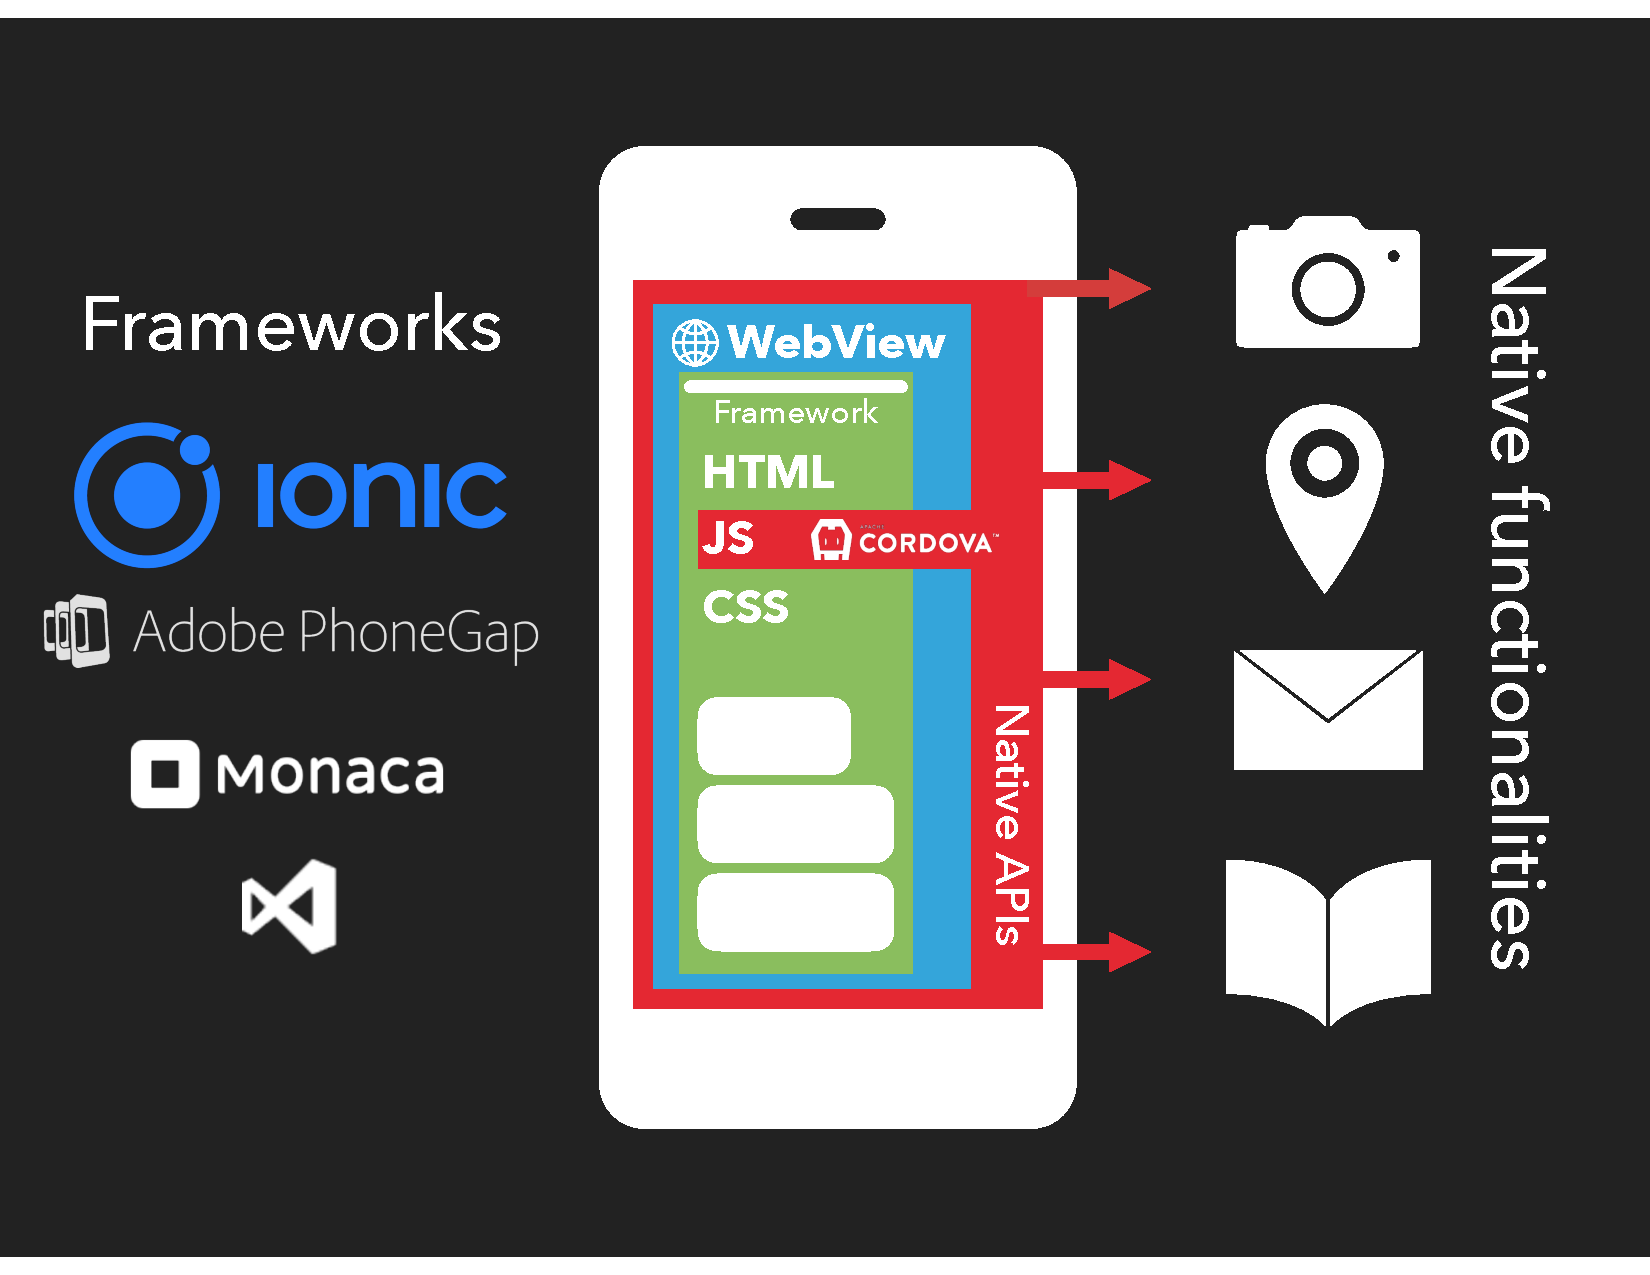
\includegraphics[width=1\textwidth]{img/hybrid.pdf}
	\vspace{-0.8cm}
	\caption{Contrary to native applications, Apache Cordova based applications contain just one activity. This activity has a basic layout with a central element: a \textit{Web view}}
	\label{hybridCordova}
\end{figure} 


Because of the differences between React Native and Apache Cordova, some argument that React Native is not hybrid. Given the fact that React Native apps can be crawled as native applications, henceforth, when we refer to hybrid applications we will refer exclusively to apps that use a Web View to present the GUI.

\subsection{Testing  hybrid applications}

Most of the research conducted in hybrid applications is focused in two categories: Debugging and Security.

\subsubsection{Debugging}

The most popular tool for debugging hybrid applications and remote web views is Chrome Developer Tools \cite{cdt}. These tools are directly built into the Google Chrome browser. Accessing to \texttt{chrome://inspect} displays the lists of web views in the devices connected through ADB. Once the browser is remotely inspecting the web view, all the errors, crashes and logs from JavaScript are printed in the computer's console. With Google Chrome, developers have access in real time to the DOM elements, network settings, and JS console to profile and audit the applications performance.

The first remote debugger was introduced in 2010: winre (WEb INspector REmote)\cite{weinre}. It was part of the Apache Cordova project, however it is being deprecated due to the increasing functionality of the Google Developer Tools. There are tools based on Google Developer Tools that enhance debugging functionality, such as the Monaca Debugger\cite{monacaDebugger} which include Cordova Plugins Supoprt and collaboration tools.


There is an approach to debug hybrid applications based on static analysis: HybriDroid\cite{7582763}.  It includes a built in bug detector based on a call graph which founds 4 types of bugs: MethodNotFound (when a JavaScript method call cannot find any target Java method to call), TypeOverloadedBridgeMethod (when JavaScript tries to use Java overloading), NotCompatibleTypeConversion (when a JavaScript type is not compatible with Java), and MethodNotExecuted (when a Java method returns an Array)\cite{7582763}.

\subsubsection{Security}

Tools and techniques related to security, are relevant to our approach because they examine the web view, and are able to analyze properties of hybrid applications.

This has been an important research topic in hybrid applications because of the possibilities of \textit{cross-language code injection}. Jin \textit{et al.} \cite{Jin:2014:CIA:2660267.2660275} define that this problem is inherited from Cross-Site scripting (XSS); additionally to their study, they developed a vulnerability detection tool.  These vulnerabilities have been detected, and numerous tools to report them have been created: NOFRAK \cite{georgiev_jana_shmatikov_2014}, Draco \cite{Tuncay:2016:DSU:2976749.2978322}, \cite{10.1007/978-3-319-27659-5_22}. Some of these approaches are based on instrumentation to  reduce the attack surface \cite{Shehab:2014:RAS:2688412.2688417}. BridgeTaint\cite{8410576} is 'a bi-directional dynamic taint tracking method that
can detect bridge security issues in hybrid apps' \cite{8410576}. It analyzes privacy leaks and code injection when the app uses bridge communication dynamically. Another tool that addresses this problem is HybriDroid\cite{7582763} which additionally to the bug detector, detects taints and leaks between Java and JavaScript. In comparison, BridgeTaint is able to detect security issues of apps built with frameworks, when HybriDroid sometimes do not.

Another topic related to security is the detection of SSL errors, Zuo  \textit{et al.} \cite{Zuo:2015:ADS:2714576.2714583} present an approach to detect statically and dynamically vulnerabilities of this kind.

\subsubsection{GUI ripping tools}

As described above, GUI ripping tools for native apps are diverse and numerous, however, as of today, there is not a single approach that focuses on GUI ripping or crawling based on hybrid applications (based on a web view). Some of the tools mentioned in section \ref{native:ripping} could work because of their implementation and the dynamic detection of components, nevertheless, they have flaws detecting different states and crashes.



 % INCLUDE: related work
\chapter{Proposed Approach}
\label{chapter3}
Before describing the proposed approach we clarify the meaning of context, domain, usage, and GUI models. A domain model describes data, entities and their relationships in an application; it looks like a network of interconnected objects, where each object represents meaningful entities and concepts. Information in a domain model is useful to determine inputs and outputs in an application under test. A graphical user interface model (GUI) is also an informative model that represents all the graphic components and views of an application, and the events that trigger transitions among the views; it is commonly represented as a state diagram and it has been widely used for GUI ripping \cite{amalfitano_fasolino_tramontana_carmine_memon_2012}. A context model \cite{crashscope} represents the surrounding conditions in which an app runs; in the case of mobile applications, it also includes sensors, networking, available hardware information (\eg device model, processor version), screen resolution and O.S version. An usage model describes how users can interact with an application and what functionalities are offered to them \cite{monkeylab}.

By augmented model (or multi-model) we mean the combination of the aforementioned models, in a single model that synthesizes relevant information.  
%A top-down approach will be used to present our approximation to augmented models for Android apps. We propose to extract a context model, a domain model a GUI model and an usage model. Our starting point is an APK and a virtual o real device. The APK can be decompiled through reverse engineering tools (\eg APK Tool \cite{apkTool}) to do static code analysis. To dynamically explore the app, we propose automated installation of the APK into a device, followed by automated exploration through ripping strategies. 
More formally, a multi-model is a directed graph. $G = (V,A)$, with
$V $ a set of states, in which each state has a unique combination of contextual variables,  GUI elements and domain entities; and 
$A$ a set of transitions, where each transition is a contextual change in the APP or an user interaction in the GUI that triggers a change in the app to a new state.

We illustrate the multi-model concept with the example presented in \figref{multimodel}; the Figure depicts an abstraction for a multi-model  generated dynamically and statically from a test app developed by the authors. The multi-model  has 3 states (\textit{S1}, \textit{S2} and \textit{S3}), and 2 edges (\textit{T1} and \textit{T2}). In this example, the app is impacted by contextual changes. %Turning off Wi-Fi in the home screen activates an alert dialog (S3) that warns the user about using bluetooth because Wi-Fi is off.  Otherwise, clicking a button in the home screen (S1) changes the app to a state where a domain element can be created by filling a text box (S2). In this scenario, a multi-model is representing a complete abstraction with domain, GUI, context and usage elements.

\begin{figure}[t]
	\centering
	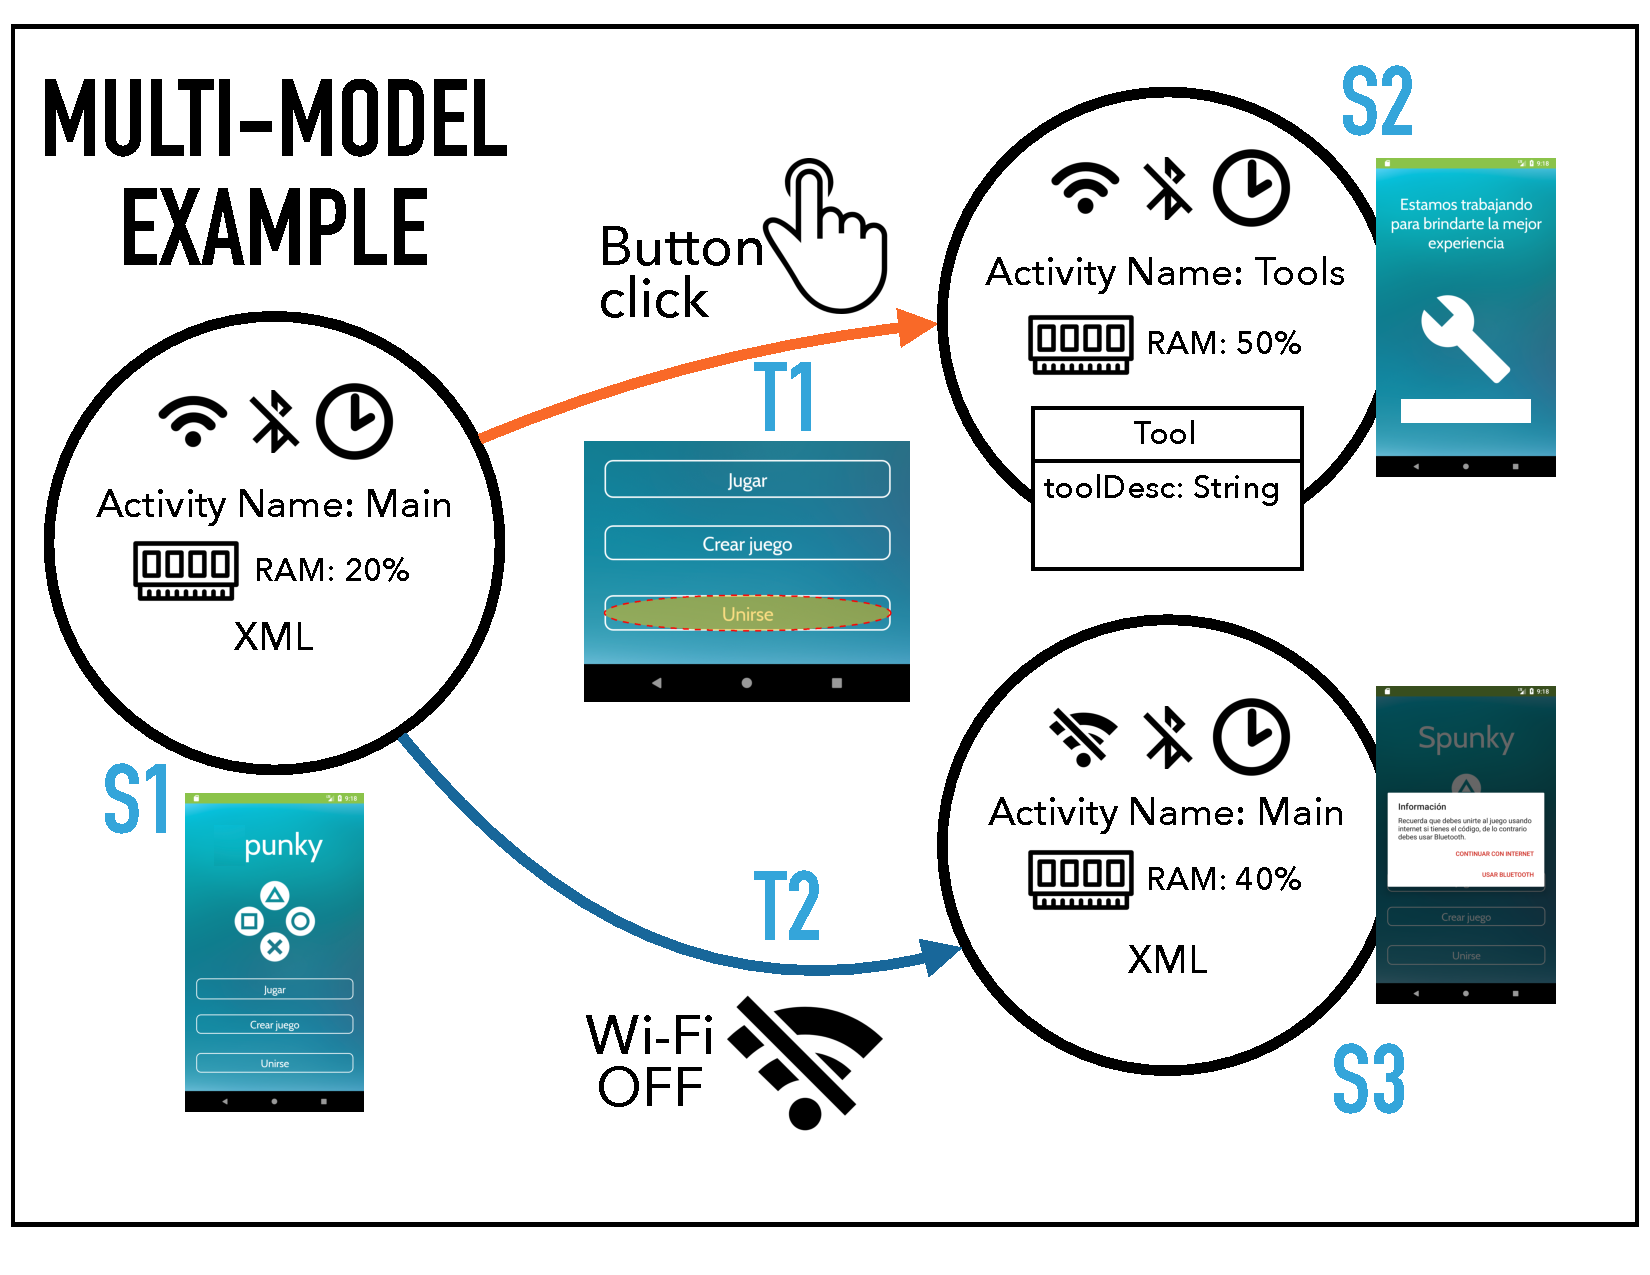
\includegraphics[width=1\textwidth]{img/multimodel.pdf}
	\vspace{-0.8cm}
	\caption{Example of multi-model generated from an Android app. The states and transitions are a subset of the complete multi-model for the analyzed app.}
	
	\label{multimodel}
\end{figure} 


\textit{S1} is the home window of the application. It is a state that mixes graphical, usage and context information. \textit{S1} occurs when Wi-Fi and cellular networks are active. On average, when this state is  active, the device has an availability of 80\% of its memory. %\textit{S1} also contains a XML screenshot of its graphical layout and an image.  
From \textit{S1}, the app flow can go to two states (\textit{S2} and \textit{S3}). The transition from \textit{S1} to \textit{S3} (\textit{T2}) occurs when Wi-Fi is turned off. \textit{S3} is a state running the same activity as \textit{S1}, however, it displays an alert message that fades out other buttons and the background. \textit{S3} is more memory greedy than the initial state.

Transition \textit{T1} changes app state from \textit{S1} to \textit{S2}. This transition is activated by clicking the button located at the bottom of the screen. Once this button is pressed, \textit{S2} is activated.  Context, graphical and usage information is also available in \textit{S2}, however, it also includes domain-related information because there is a text-input for collecting information from the user; thus, we consider the activity (\ie the Android window related to \textit{S2}) as an entity named ``Tool” with a string field called ``toolDesc”.

%Summarizing \figref{multimodel}, this example app with 3 states is affected by contextual changes. Turning off Wi-Fi in the home screen activates an alert dialog. When this alert appears, more RAM memory is being used in the device. Clicking a button in the home screen changes te app to a state where a domain element is created by filling a text box. In this scenario, a multi-model is representing a complete abstraction with domain, GUI, context and usage elements.

\section{General Approach}

\begin{figure}[t]
	\centering
	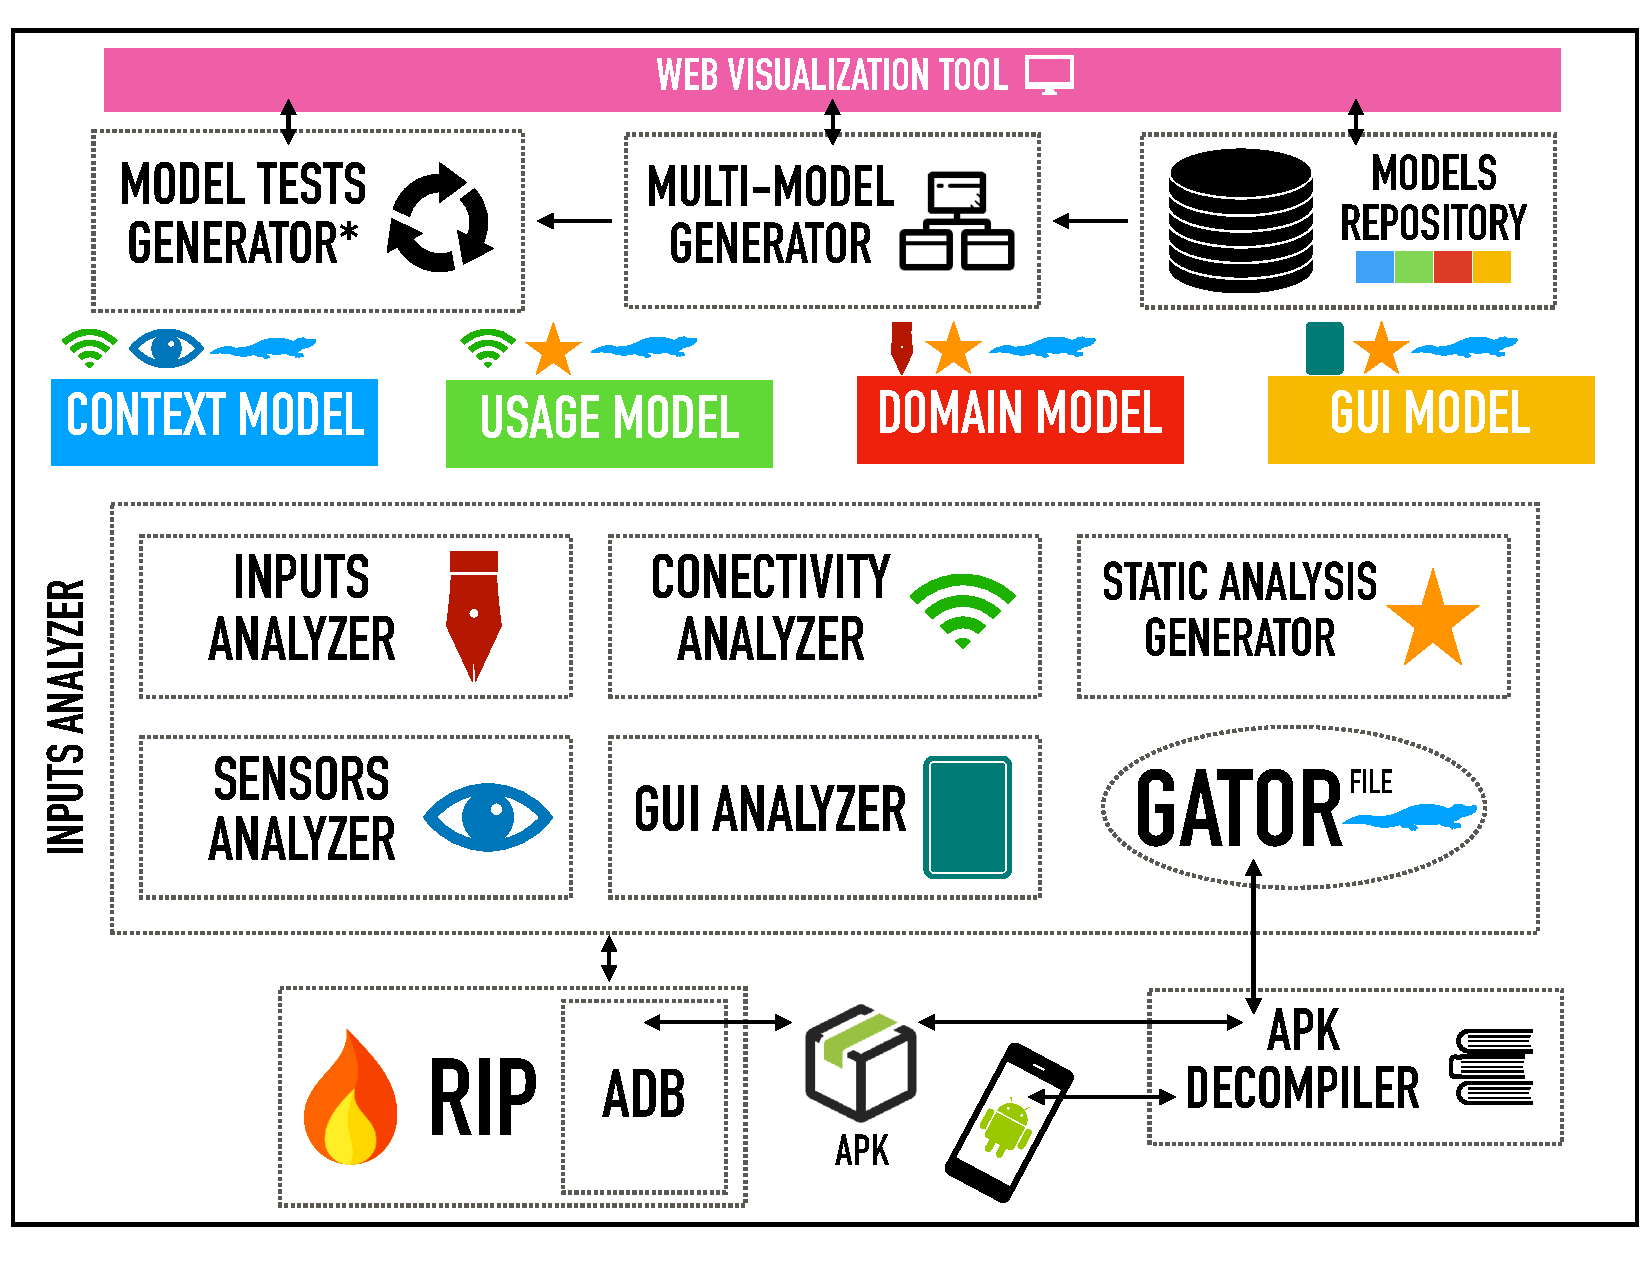
\includegraphics[width=1\textwidth]{img/generalArchitecture.pdf}
	\vspace{-0.8cm}
	\caption{Proposed architecture (\textbf{RIP}) for extracting augmented models for Android apps.}
	\label{generalArchitecture}
\end{figure}	

We have designed an  architecture \figref{generalArchitecture} that enables a series of stages that include: ripping, automatic extraction of static and dynamic models, generation of multi-models and model-based tests generation.

The multi-model generation starts by ripping the app under test. For this purpose, we have designed and developed a desktop tool called \textbf{RIP}, which is publicly available at \url{https://github.com/TheSoftwareDesignLab/rip}. It is an automation software that executes a series of actions and emulates user interactions into an Android device to extract models; this is done through the Android Debug Bridge (ADB) \cite{adb}, a command-line tool that provides access to an Android device over USB or Wi-Fi. In comparison to monkey/random testing tools that generate random interactions to find bugs and corner cases, \textbf{RIP} follows an strategy to explore the application based on the dynamic content that appears on a device screen (like other rippers do). \textbf{RIP} not only simulates user interactions in the screen; \textbf{RIP} also executes contextual changes to the application that vary the network configuration and the readings of the sensors (\eg accelerometer, gravity, gyroscope, light, proximity, magnetic field).  During the execution,  \textbf{RIP} collects GUI-related, domain-related. sensors-related, and resources-related information. In addition, screenshots and  GUI-hierarchies are collected for each state.

Our approach differs from existing ones because we are able to (i) generate a comprehensive list of contextual changes, (ii) extract a domain model from GUI states,  (iii) augment the dynamically-generated model with information collected statically, and (iv) considers exploration of hybrid applications. Due to security restrictions imposed by Android devices and the Android framework, in order to enable contextual events execution via ADB (\eg airplane mode, Wi-Fi), it is necessary to run the commands in a rooted physical device or an emulator.

\textbf{RIP} takes advantage of static code analysis to enrich the final generated model. When the ripping process finishes, RIP augments the collected model with a graph generated statically by GATOR \cite{gator}, a static reference analyzer tool for GUI objects in Android. This tool has been chosen because its context-aware approach in static code analysis \cite{yang_yan_wu_wang_rountev_2015}. GATOR finds static references to GUI components and determines its control flow. If \textbf{RIP} identifies missing states (\ie states detected by GATOR but not by \textbf{RIP}), it adds the new states to the dynamically generated model. Thus, the  GUI and usage models are represented by the combination of transitions and states information extracted from the ripping and GATOR.

GATOR code is not included in \textbf{RIP}. To combine static information with RIP's execution, GATOR analysis should be run first, and then passed to \textbf{RIP}. An example of the file that \textbf{RIP} imports from GATOR is presented in the code example \ref{gatorFile}

\begin{lstlisting}[language=json, caption={Fragment of a GATOR file obtained from a native application}, label={gatorFile}, firstnumber=1]
{ "nodes": [{
"id": 2160,
"name": "com.simplemobiletools.commons.activities.FAQActivity"
}, {
"id": 2076,
"name": "android.view.Menu"
}, {
"id": 2140,
"name": "android.view.Menu"
}, {
"id": 14106,
"name": "android.app.DatePickerDialog"
}],
"edges": [{
"source": 2076,
"target": 2140,
"event": "implicit_power_event"
}, {
"source": 14106,
"target": 14106,
"event": "implicit_home_event"
}, {
"source": 2140,
"target": 2140,
"event": "implicit_rotate_event"
}, {
"source": 2160,
"target": 2160,
"event": "implicit_home_event"
}]}
\end{lstlisting}

\section{RIP components}		

Our architecture defines a layer of analyzers that guide \textbf{RIP} during the models extraction:

\subsection{GUI analyzer}

It extracts the hierarchy of graphical components in the app. It is able to differentiate app GUI states based on the analysis of the GUI hierarchy represented as an XML file. It means, the construction of the GUI model is done iteratively, according to the app exploration. To determine if two views are different, a decision process is followed. Firstly, if the activity names differ from each other, the two views are classified as different states. Otherwise, if the activity names are the same, then the XML is analyzed; each view is compared by the number of elements, checked boxes,  buttons, labels content, alerts, and messages.  In the case of menus or dialogs that are displayed on a view, we consider them also as states.

\begin{lstlisting}[language=xml, caption={XML dump from an app, containing the layout hierarchy},label={xmlDump}]
<?xml version='1.0' encoding='UTF-8' standalone='yes' ?>
<hierarchy rotation="0">
<node index="0" text="" resource-id="" class="android.widget.FrameLayout" package="com.clockwork.mcdonalds"
content-desc="" checkable="false" checked="false" clickable="false" enabled="true" focusable="false" focused="false"
scrollable="false" long-clickable="false" password="false" selected="false" bounds="[0,0][1080,1794]">
<node index="0" text="" resource-id="" class="android.widget.LinearLayout" package="com.clockwork.mcdonalds"
content-desc="" checkable="false" checked="false" clickable="false" enabled="true" focusable="false"
focused="false" scrollable="false" long-clickable="false" password="false" selected="false" bounds="[0,0][1080,1794]">
<node index="0" text="" resource-id="android:id/content" class="android.widget.FrameLayout" package="com.clockwork.mcdonalds"
content-desc="" checkable="false" checked="false" clickable="false" enabled="true" focusable="false"
focused="false" scrollable="false" long-clickable="false" password="false" selected="false" bounds="[0,63][1080,1794]">
<node index="0" text="" resource-id="" class="android.widget.ImageView" package="com.clockwork.mcdonalds"
content-desc="" checkable="false" checked="false" clickable="false" enabled="true" focusable="false"
focused="false" scrollable="false" long-clickable="false" password="false" selected="false" bounds="[0,63][1080,1794]" />
</node>
</node>
<node index="1" text="" resource-id="android:id/statusBarBackground" class="android.view.View" package="com.clockwork.mcdonalds"
content-desc="" checkable="false" checked="false" clickable="false" enabled="true" focusable="false"
focused="false" scrollable="false" long-clickable="false" password="false" selected="false" bounds="[0,0][1080,63]" />
</node>
</hierarchy>
\end{lstlisting}

%Some thresholds can be configured by the developer to change the sensitivity of states detection. 

The set of states gathered from visual information are the source for the GUI model. \textbf{RIP} captures image screen-shots and  XML layouts from every state it has found. It also records the interaction/event that triggered the state transition (\eg pressing a button); note that state transitions are modeled as edges connecting states. To extract the XML layout information, \textbf{RIP} executes the command \verb|adb shell uiautomator dump|. Eventually, the device stores this dump into an XML file such as the code example \ref{xmlDump}. Because this file is stored in the SD card, it must be extracted and parsed in the host computer. To capture the image snapshot of the device, a remote screen-shot is invoked with the command \verb|adb shell screencap|. All the files in the devices are extracted through \verb|adb pull|.

%The GUI model finally will be shown as a state diagram, including transition as edges connecting different states of the application.


\subsection{Inputs analyzer}

It enables \textbf{RIP} to identify user input-related GUI Android components and interact with them accordingly (\eg check boxes, text boxes, lists, scrollable views).  \textbf{RIP} creates random input data for the components based on the input types defined for text fields, and the component nature (\eg a check box can be activated or deactivated). Keyboards that appear on the screen and GUI components meta-data, give us clues about concepts and domain entities that are part of the domain model of the application. 
We define entities of the domain model as views that have input elements. Each entity has a set of attributes that correspond to input-related components in the view, and the attributes type is inferred from the type of input allowed (\eg numbers, special characters, boolean check, lists, \etc). 

\subsection{Sensors analyzer}

During the ripping, \textbf{RIP}  turns off/on sensors, randomly. The sensors analyzer identifies which sensors the application has access to from the app's manifest file. Once the sensors analyzer has this information, it detects the states where sensors are on and off using specific ADB commands. 

To obtain a detailed list of sensors, \textbf{RIP} invokes the command \texttt {adb shell pm list features}. The available sensors in the device are listed as features (\eg \verb|hardware.camera|,  \verb|hardware.sensor.gyroscope|, \verb|hardware.sensor.light|)

\subsection{Connectivity analyzer}

This component identifies connectivity status of the app during all the ripping execution. Once the GUI has detected an initial set of states, it sends requests to the device in order to control Bluetooth, Wi-Fi, celullar networks and airplane mode. \textbf{RIP} triggers connectivity changes in every view of the application. If an error occurs or the GUI changes after the contextual change, then a new state is  discovered and added to the model.

To determine the connectivity settings of the device, \textbf{RIP} calls the command \texttt {adb shell dumpsys wifi | grep 'Wi-Fi is'} to determine Wi-Fi status, \texttt {adb shell dumpsys wifi | grep 'mAirplaneModeOn'} to determine Airplane Mode, etc. The activation or deactivation of these settings is done with the commands  \texttt {adb shell svc wifi (disable|enable)}, \texttt {adb shell svc bluetooth (disable|enable)}, \texttt {adb shell svc data (disable|enable)}, etc. Commands that enable or disable connectivity settings of the device require root privileges.


\subsection{Static analyzer and GATOR}
Different from the other components, it imports a flow graph of the app based strictly on static analysis, by relying on the GATOR tool \cite{gator}. GATOR creates a window transition graph with activities, dialogs and menus. The transitions of the graphs include events such as button pressings and window stack operations (push and pop). This flow graph is used to augment the model collected dynamically by  \textbf{RIP}, in particular to have a more comprehensive list of transitions and states. This graph is presented in the code example \ref{gatorFile}.

%	\begin{figure}[h]
%		\centering
%		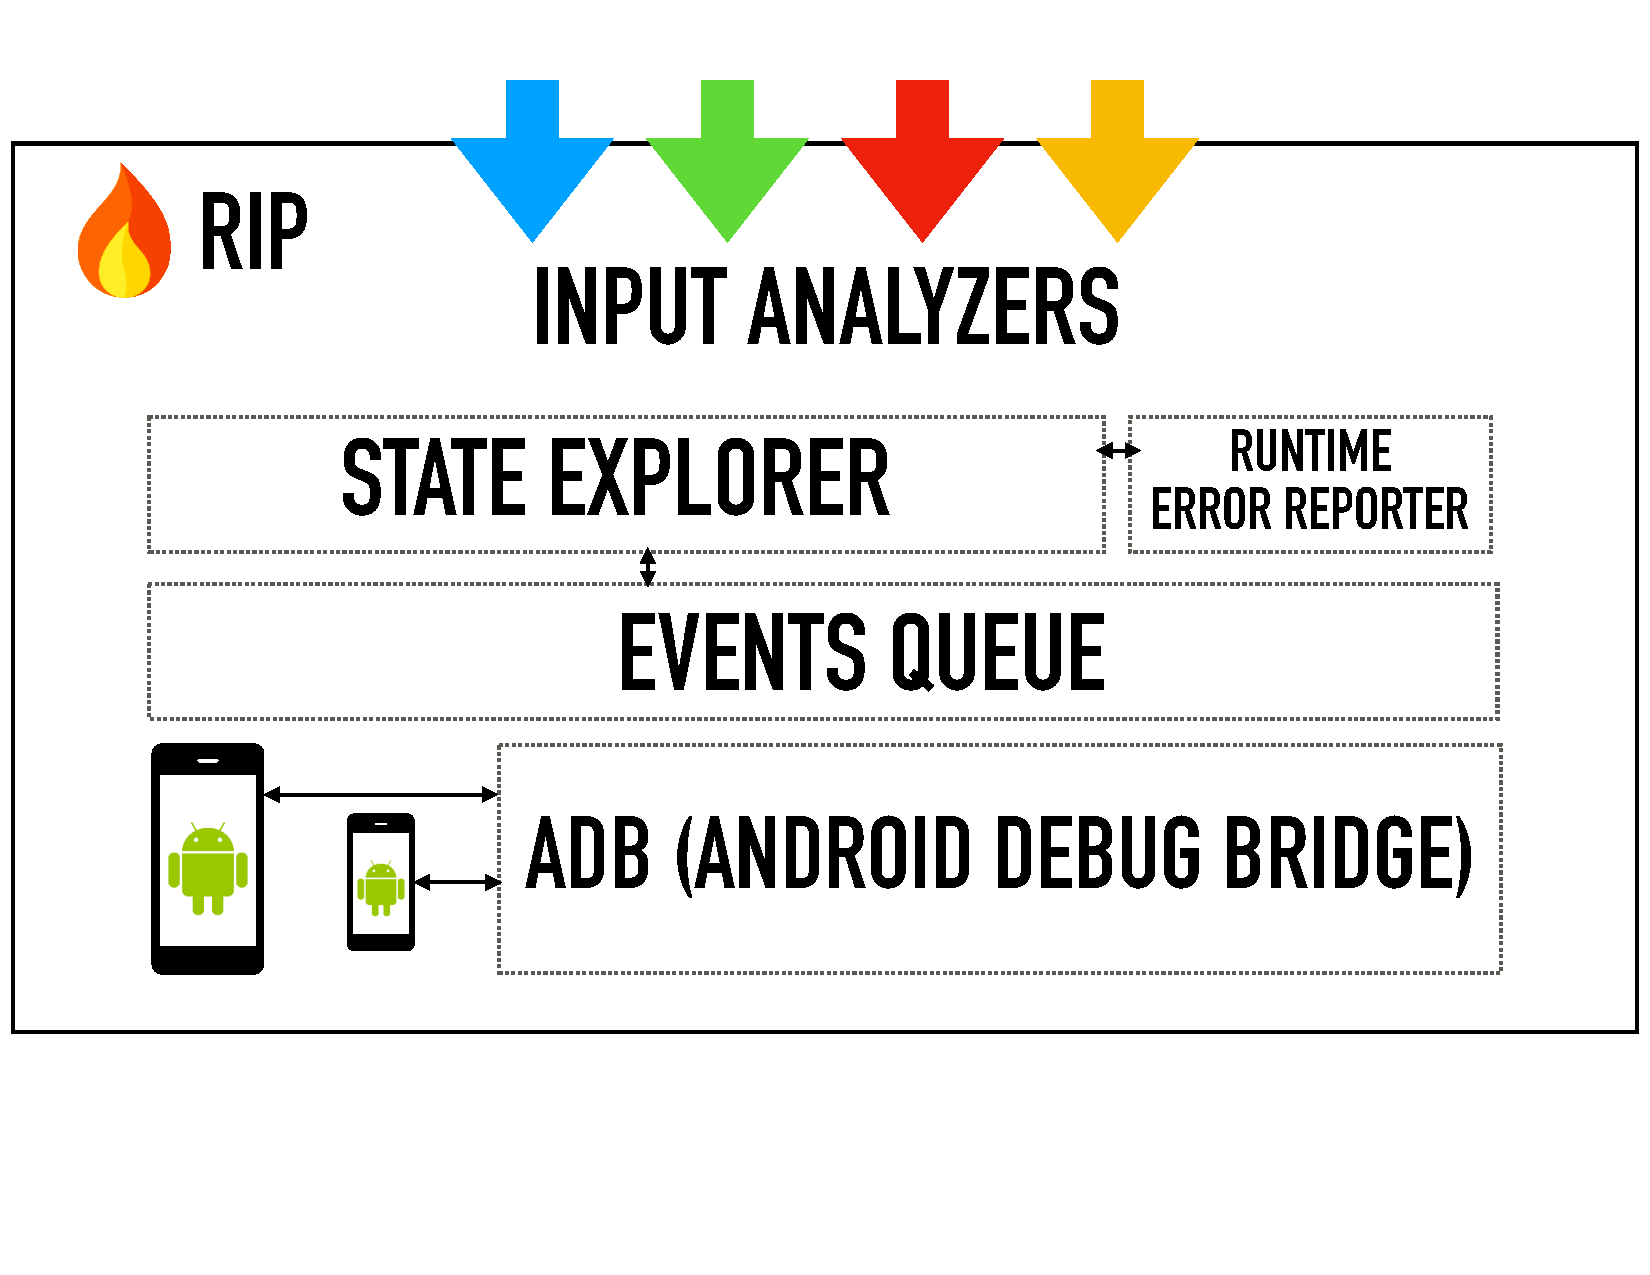
\includegraphics[width=0.5\textwidth]{img/ripArchitecture.pdf}
%		\caption{RIP components.}
%		\label{ripArchitecture}
%	\end{figure} 
%	

\subsection {RIP GUI}
It interacts directly with ADB to explore the applications dynamically and coordinates the execution of the other components. The \textbf{RIP} GUI combines the ripping, interactive data collection, and static analysis, to generate individual models and a multi-model like the one presented in \figref{real}; the \textbf{RIP} GUI also generates the model as a JSON file that can be analyzed by any other tool.

%\textbf{RIP} identifies native graphical Android elements to explore systematically every possible view of the app. This tool is able to simulate user interactions and contextual changes. RIP sends the gathered information to all the analyzers in order to build the mentioned models. \figref{real} presents a multi-model generated from our test app.

\begin{figure}[t]
	\centering
	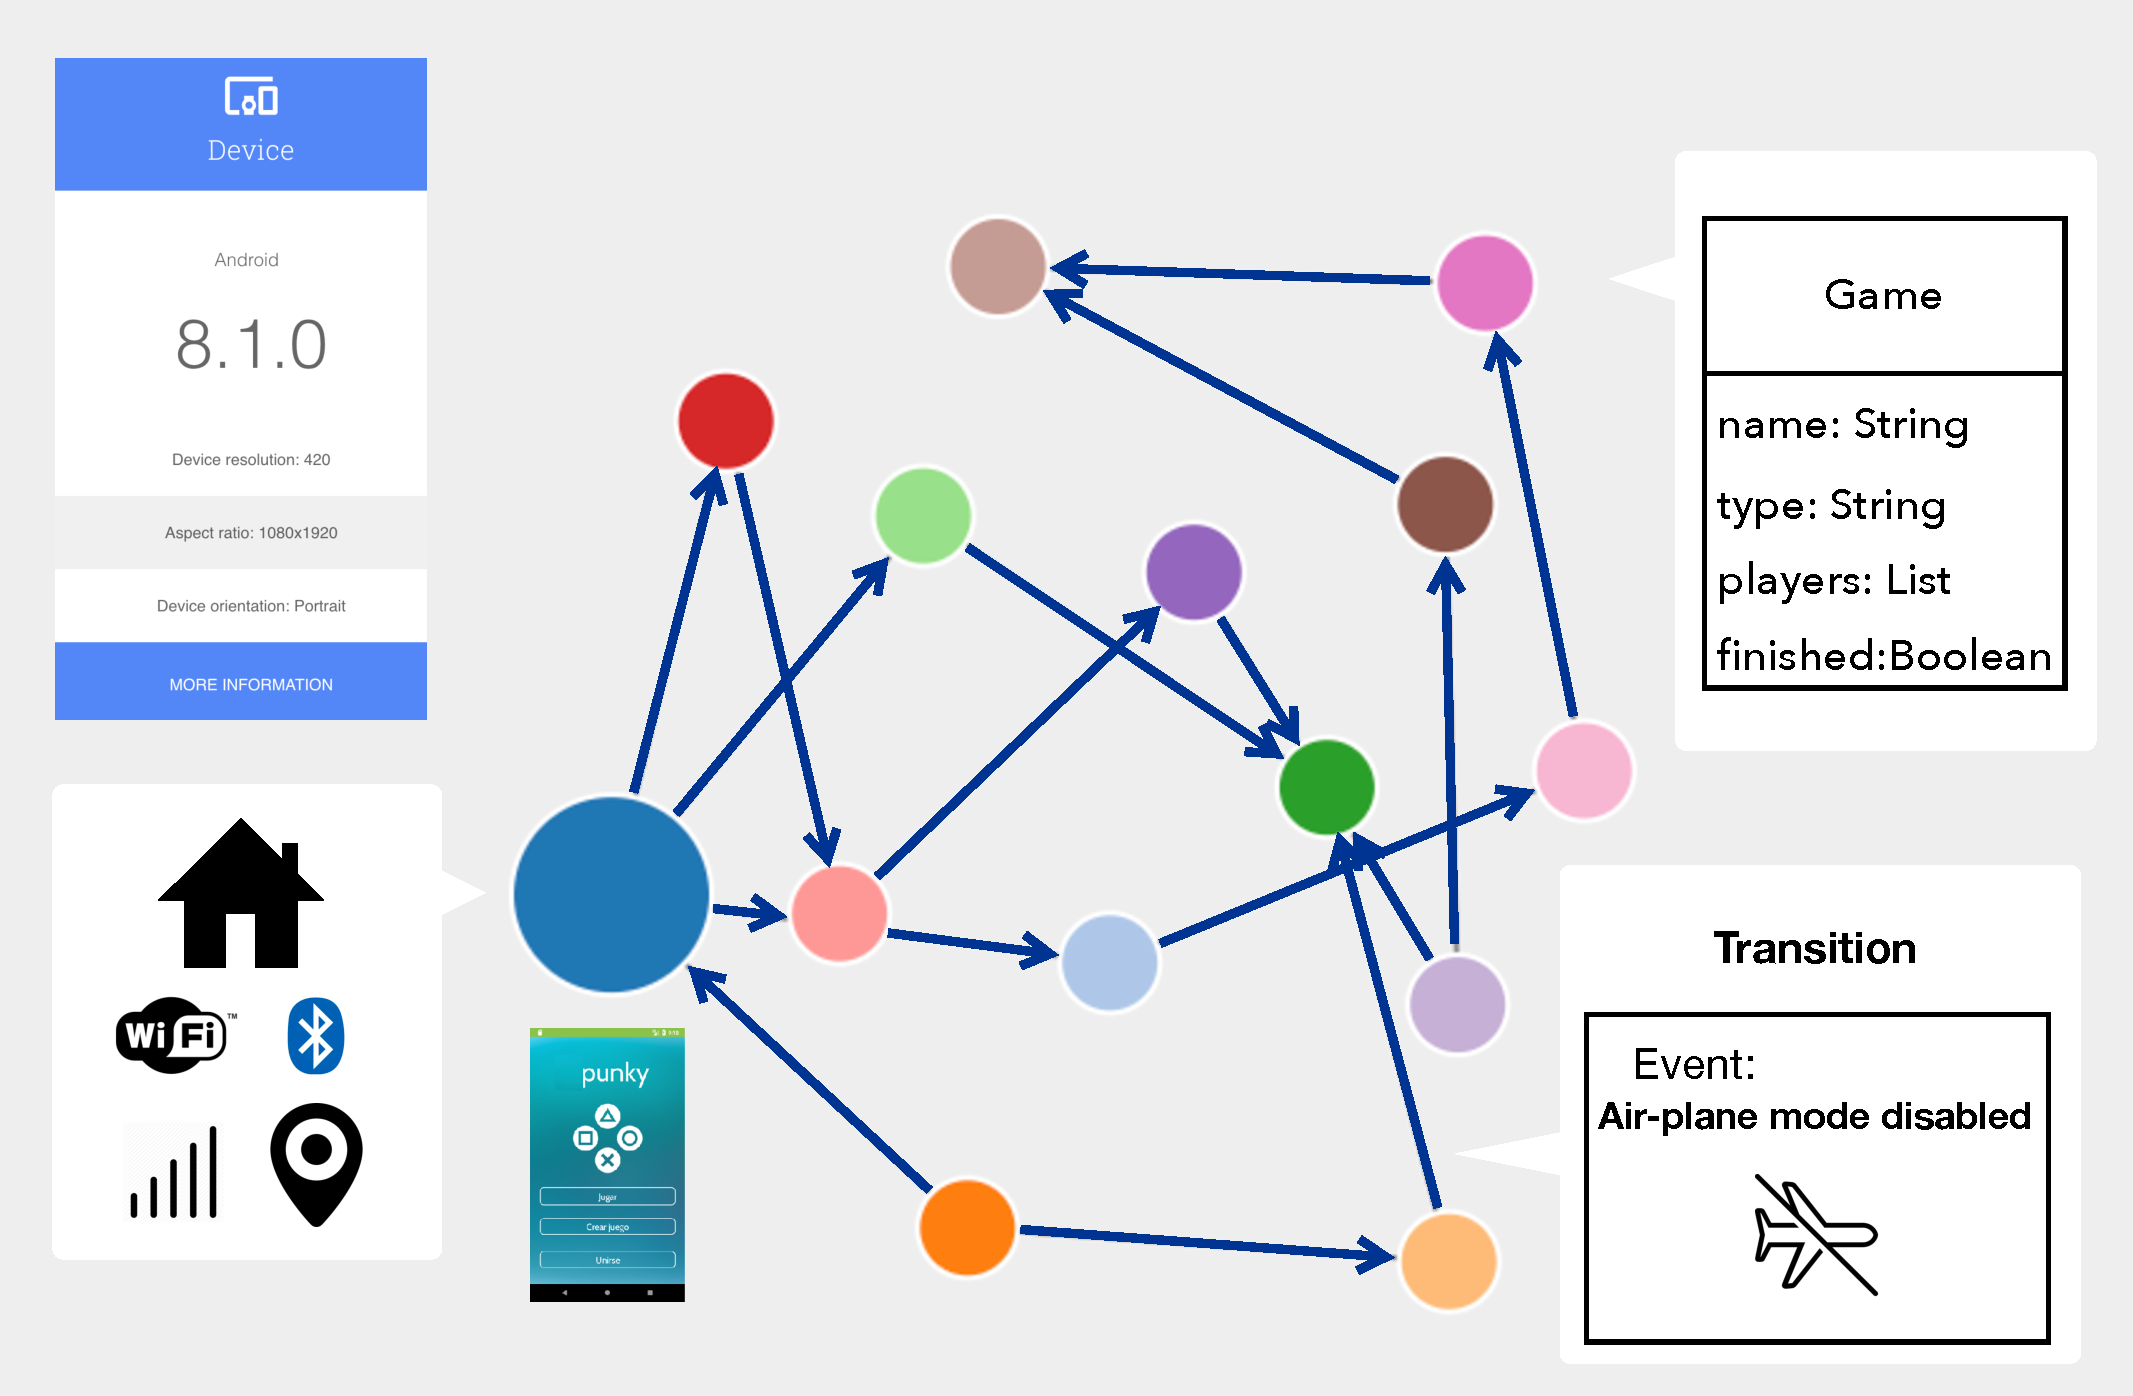
\includegraphics[width=1\textwidth]{img/multimodel-real.pdf}
	\vspace{-0.8cm}
	\caption{Example of multi-model created by RIP.}
	\label{real}
\end{figure} 

%	RIP general architecture is presented in \figref{ripArchitecture}. RIP communication with the device is done through Android Debug Bridge (ADB).
%	
%	\subsubsection{Events Queue}
%	RIP has an events queue that manages and synchronizes events between ADB and the state explorer. 
%	
%	\subsubsection{State explorer}
%	The states explorer is the controller of the automated interactions against an application. Once an APK is installed in a device, it defines the exploration strategy that RIP will follow. Input analyzers send request to the state explorer to push and pull information from the headset.
%	
%	Exploration could follow two principles. First, random exploration introduces random interactions into the app. These interactions include GUI analyzer interactions (\eg pressing random buttons, selecting check boxes, swiping), Input analyzer interactions(\eg Introducing text strings, numbers), connectivity interactions (\eg enable airplane mode, disable Bluetooth) and sensors interactions (\eg simulate a move of the accelerometer). This exploration method can be executed until a number of interactions have been done or until a timer ends.
%	
%	Second principle of exploration is guided exploration. It includes the same interactions, but this time it sets itself the objective of explore and cover the maximum amount of possible states. This kind of exploration is done by DFS and request the analyzers to create all the possible configurations for each view changing connectivity and sensors informations.
%	
%	\subsection{ Models repository}
%	
%	Models repository condenses all the generated models to be processed by the multi-model generator.
%	
%	\subsection{Multi-model generator}
%	
%	The multi-model generator takes as input the context, usage, domain and GUI models and combines all the models into a richer sate diagram.
%	
%	%\subsection{Test generator}
%	
%	%Test generator is currently not developed, however, it is a future step that will enable model-based testing based on the multi-model generation.
%	
%    \subsection{WEB visualization tool}
%    
%    Finally, a web visualization tool based on Javascript, HTML and D3 presents the final  multi-model. All the intermediate models are also included. This tools is presented in \figref{webTool}.
%    
%    \begin{figure}[h]
%    	\centering
%    	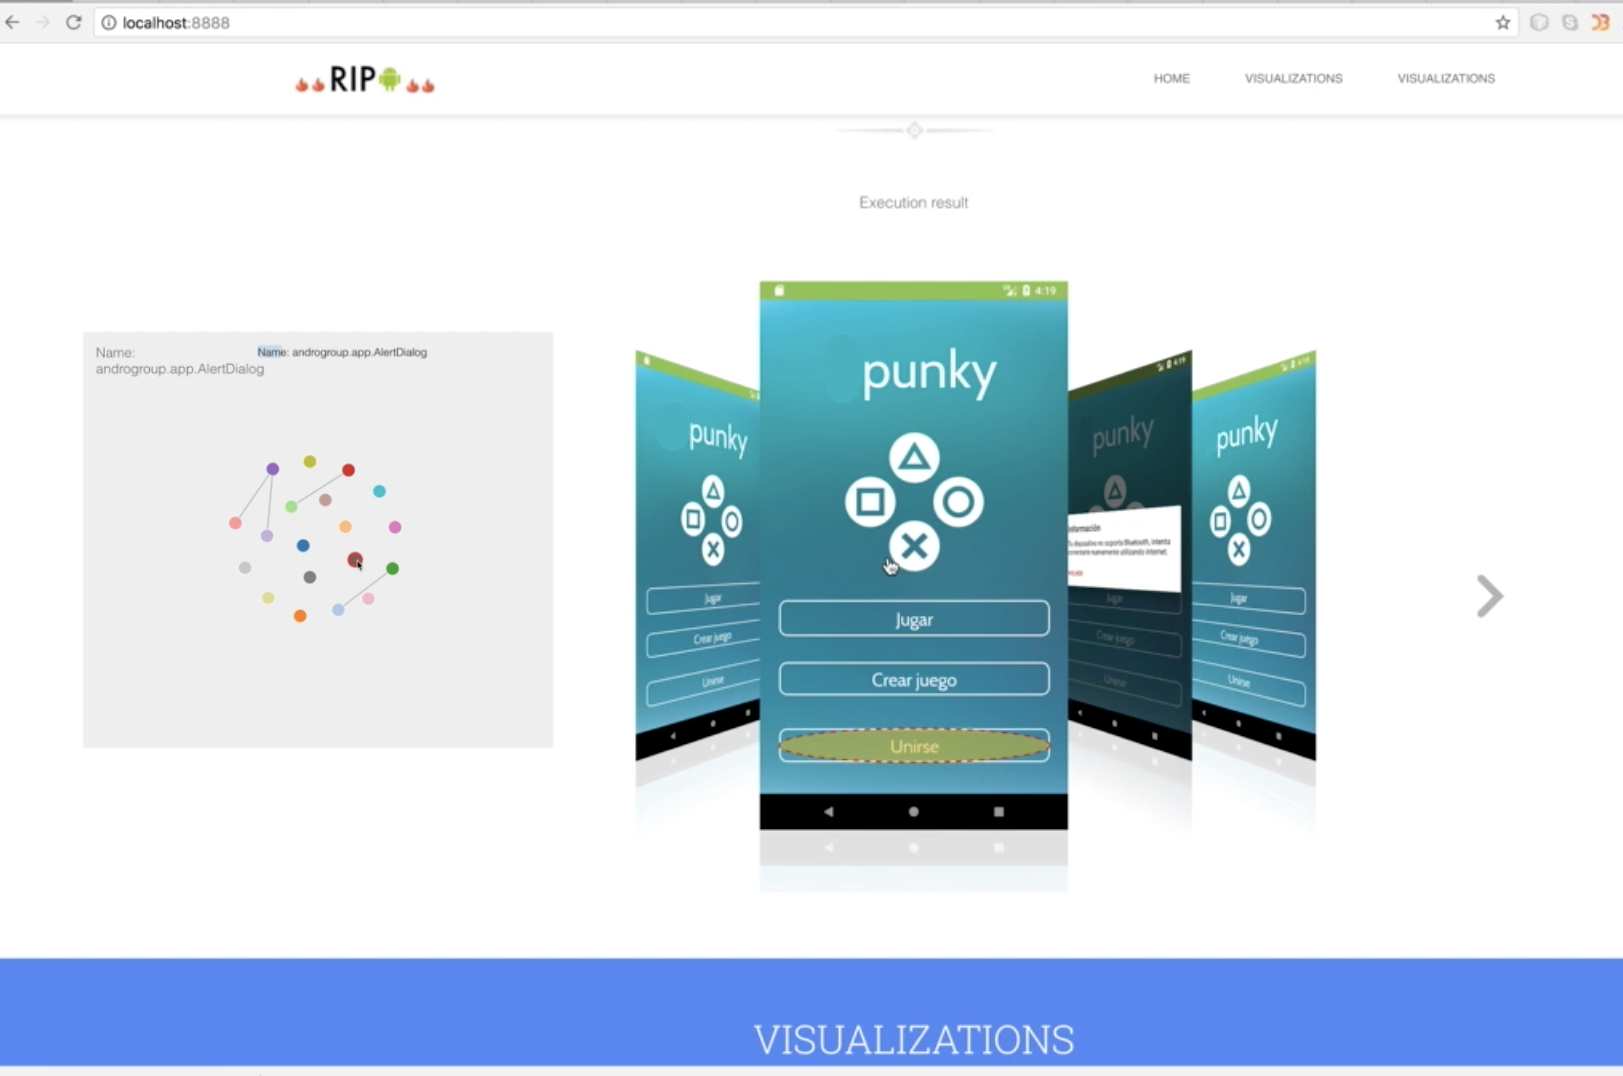
\includegraphics[width=0.5\textwidth]{img/webTool.png}
%    	\caption{WEB visualization tool}
%    	\label{webTool}
%    \end{figure} 

\section{Ripping  hybrid applications}
As described before, hybrid apps are those in which developers write significant portions of their application in cross-platform web technologies, while maintaining direct access to native APIs when required \cite{ibmHybrid}. This way of developing applications is gaining popularity among the mobile developers community because:
\begin{itemize}
	\item Reduces the time to develop cross platform apps
	\item It is based on Web technologies, which allows developers to recycle modules and components from existing Web developments
	\item Browser engines are becoming faster and mobile devices more powerful
	\item Performance differences between native and web technologies are becoming imperceptible
\end{itemize}

Currently, Apache Cordova is the component that enables the access to native iOS and Android APIs from the JS code. This piece of software gives access to Local Storage, Camera, GPS, and all the available sensors of each platform. Apache Cordova is the core of many popular hybrid frameworks such as Ionic, Adobe Phonegap, Monaca or Visual Studio. 

\subsection{Barriers for ripping hybrid apps }
Ripping native apps is different from ripping hybrid apps. The main reason is the underlying techonologies; in native apps the GUI is rendered by the view system and window manager of the  framework, in hybrid apps the GUI and events are managed by a Web View. In native applications, a native layout defines the structure of the user interface. An activity contains a hierarchy of containers and graphical objects called \textit{Views} and \textit{View groups}. These objects are also known as \textit{widgets}. Widgets could be instanced as elements such as buttons, labels, text fields, among others. View groups provide the structure of widgets and other view groups in the screen \cite{layouts}. To crawl dynamically apps, this hierarchy must be extracted continuously, and based on the layout information, the ripper can execute commands and simulate user interactions.

Contrary to native applications, most hybrid applications contain just one activity. This activity has a basic layout with a central element: a \textit{Web view} \cite{webView}. Web views are widgets that can render web content \figref{hybridCordova}. When the user interacts with elements of the web view, the JavaScript engine is in charge of changing the view. All the application logic is entirely written in JavaScript, therefore, errors, bugs and crashes are only visible to the web console. Additionally, the HTML DOM is not visible through the \verb|adb dumpsys| command.

\subsection{Strategies for ripping hybrid apps }
In \textbf{RIP}, we have defined and implemented a series of strategies designed to tackle the ripping of hybrid apps. Specifically, we consider important to maximize the coverage of states discovered and enable detection of crashes, while maintaining the  strategy of multi-model extraction and contextual exploration. 

\subsubsection{Detecting crashes in hybrid apps}
Crashes are usually the result of uncaught exceptions. Other crashes come from ANRs (\textit{Application Not Responding}), permission denials, network errors, and bad practices. These kind of crashes are well defined in the Android Developers Documentation and if one of them occurs, it is reported in the device. When one of these crashes is thrown, rippers of native apps are able to recognize them because the device writes them in the device log (logcat). In general, hybrid applications do not deal with these errors as native applications do, because their errors  are written in the JS console. In order to capture errors in hybrid applications, RIP reads continuously the WebView console with the help of Chromium.

While \textbf{RIP} crawls a hybrid application, it listens to the web console, and stores the web errors associated with each state. As these errors occur in an embedded web browser, all the HTTP errors can be associated to the running application. %As an example, in Figure \ref{hybridError} is depicted a 503 HTTP status code: Service unavailable.

\subsubsection{Maximize the coverage of states discovered}
In order to maximize the coverage of states discovered, \textbf{RIP} must interact with every 'clickable' element inside the web view. The exploration should not be focused on finding and interacting with Android widgets, but with every new component accessible in the web view. A better approximation to explore the hybrid GUI should extract and parse the DOM of the web components with the help of the Chrome inspector, however, this is considered as future work.

We found experimentally that introducing some randomness to the ripping process in these applications improves the discovering of new states, because not all the web elements can be extracted solely with UIAutomator, and always remains actions of the application that could not be accessed systematically.

Finally, a key step that improves exploration of hybrid apps is triggering contextual changes, specifically, toggling network and Internet settings. This occurs because sometimes, all the web view content is not served just from the mobile device, but also from external servers in the Internet. Hybrid applications are highly prone to errors due to contextual changes.

\begin{lstlisting}[caption={Pseudocode describing the Ripping process},label={pseudocode}]
transitions = []
discoveredStates = []
contextualChanges = [rotateScreen, turnOnWifi, ...]
func explore(t):
	s.clickOrExecute()
	transitions.push(s)
	if thisIsANewState():
		discoveredStates.push(currentState)
	if state.hasClickableElementsLeft():
 		for everyClickableElementInState c:
     		if c has not been clicked:
         		explore(c)
 	elif !state.hasClickableElementsLeft() and !state.contextualChangesDone():
 		for every cc in contextualChanges:
 			explore(cc)
 	elif state.ContextualChangesDone()
 		if state.isHybrid():
 		 	enableJSConsole()
 			action = randomAcctions()
 			explore(action)

\end{lstlisting}

	% INCLUDE: system
\chapter{Empirical study}
\label{chapter4}
The \textit{goal} of our empirical study is to evaluate the proposal of combining multiple models to improve accuracy of testing processes and to evaluate \textbf{RIP} as a tool to automatically crawl Android applications. We evaluate our proposal in terms of (i) the importance of combining orthogonal information from different models and (ii) the suitability of a multi-model testing tool, in the process of developing mobile applications. At the same time, we evaluate \textbf{RIP} in terms of (iii) RIP's ability to crawl native and hybrid Android apps, and (iv) RIP's ability to detect bugs and generate crashes. The \textit{context} of this study consists of (i) a set of 15  open source native APKs, (ii) a set of 20 hybrid APKs from the Google Play Store, and (iii) three baseline approaches for extracting models and crawl Android applications: DroidBot \cite{Li:ICSE17}, Firebase Test Lab Robo \cite{firebase} and Monkey \cite{monkey}.

The \textit{quality focus} of this study is the effectiveness of \textbf{RIP} to detect  states on both native and hybrid apps, reporting crashes and generating multi-models from these applications. To aid in achieving the goals of the study, the following research questions were formulated:

\begin{itemize}
	\item \textit{\textbf{RQ$_1$}}: \textit{Is the combination of multiple models useful to gather more information of an app under test?}
	\item \textit{\textbf{RQ$_2$}}: \textit{How accurate is the state discovery algorithm' implemented in RIP when compared to state-of-the art tools?}
	\item \textit{\textbf{RQ$_3$}}: \textit{Is RIP suitable to detect crashes and bugs in Android apps?}
\end{itemize}
 
Note that when answering the research questions we take into account hybrid and native Android apps. These two development strategies could be indistinguishable for final users of the apps, yet their are very different to crawl, analyze and build. \textbf{RIP has been designed to support both types of apps.}

\section{Context of the study}

A set of 15 native Android apps and 20 hybrid apps were downloaded from the Google Play Store and F-Droid. The native apps were randomly selected from F-Droid. In order to identify and download the set of hybrid apps, it was necessary to check the different hybrid frameworks showcases, find the APKs in the Google Play Store and then decompile the APKs to identify the presence of hybrid packages (\eg \verb|com.ionicframework|). Additionally, to verify that these apps contain web based GUI elements, the \textit{Show layout bounds} setting was activated in a device. With this option enabled, it is possible to visually identify native Android components in a device screen. Figure \ref{layoutBounds} shows that in native apps, this option draws red and blue lines around every graphical element. On the other hand, it can be seen that when this option is enabled in a hybrid app, none of these components is detected by the layout manager.

\begin{figure}[t]
	\centering
	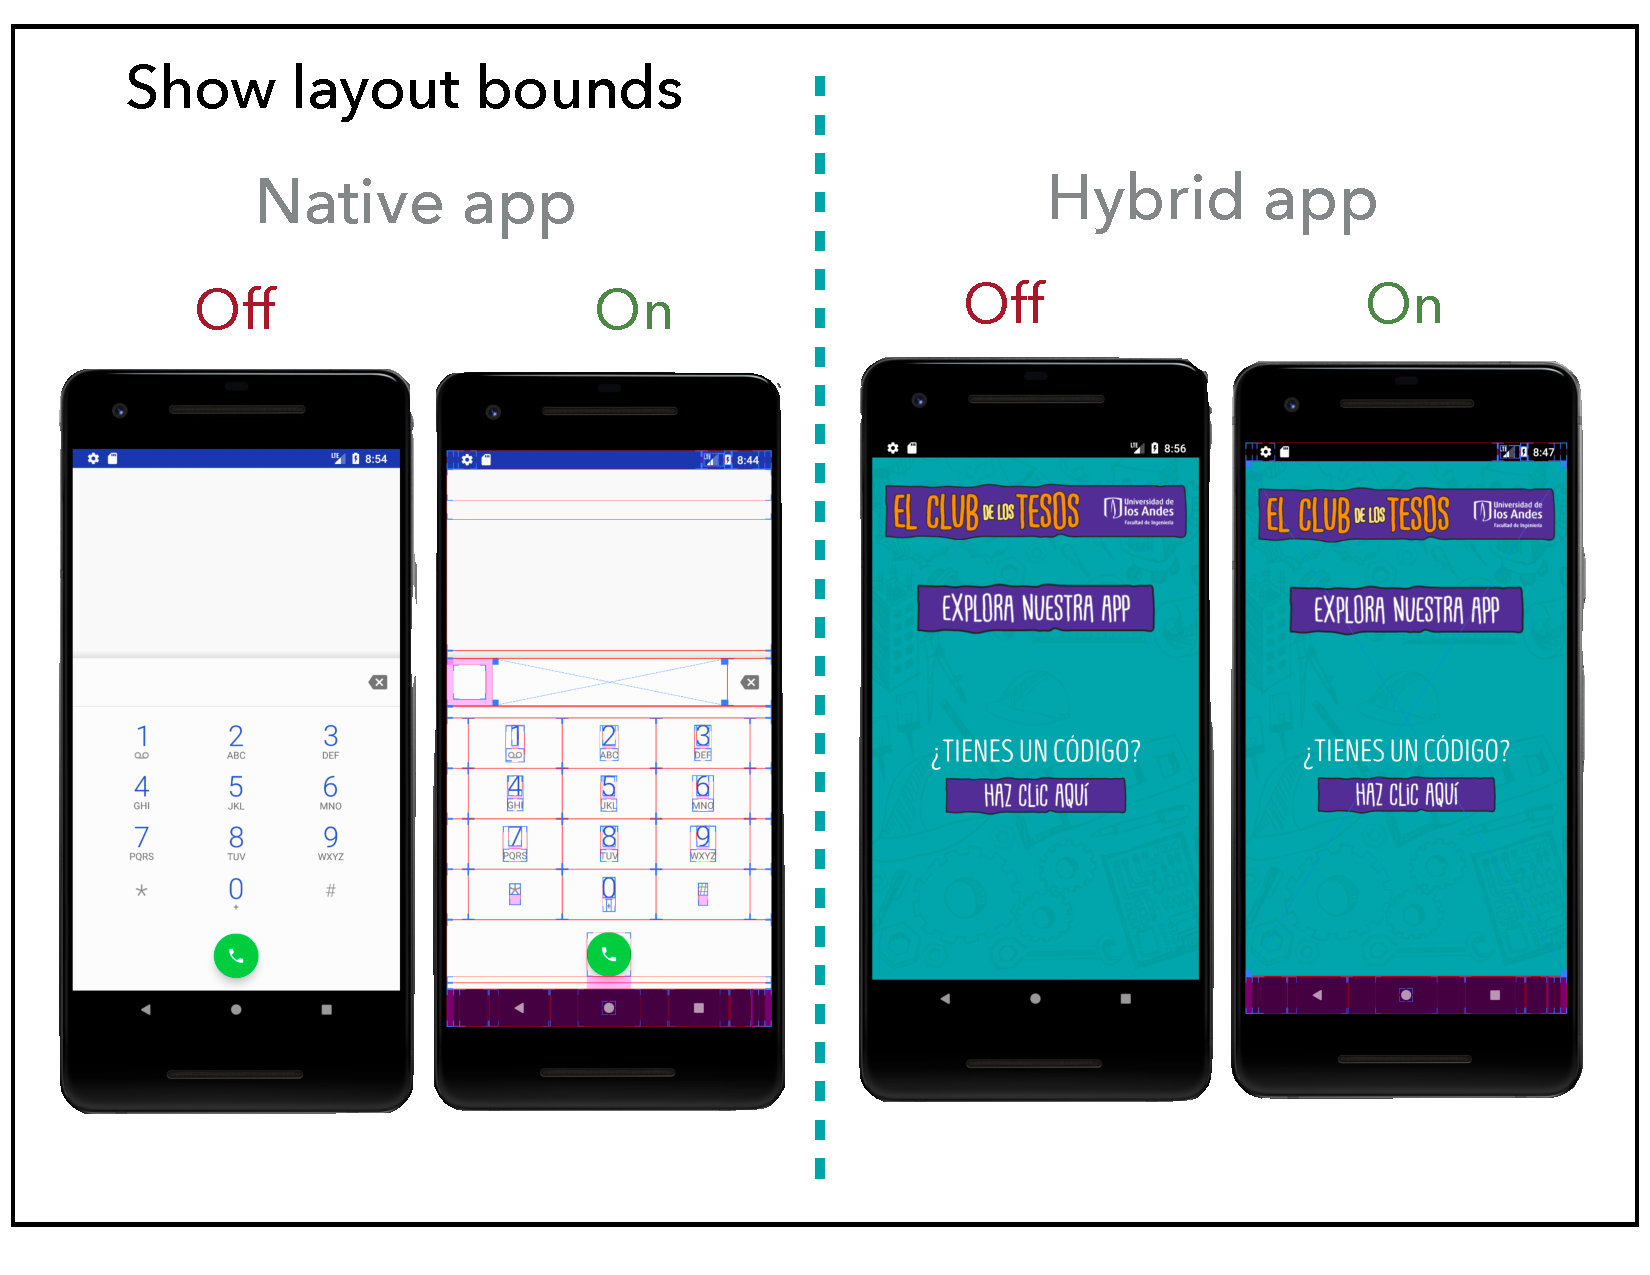
\includegraphics[width=1\textwidth]{img/layout.pdf}
	\vspace{-0.8cm}
	\caption{Enabling layout bounds detection in hybrid and native apps}
	\label{layoutBounds}
\end{figure} 


All the applications were installed and tested in an Android emulator for a \textit{Pixel 2} device with API 27 (Android 8.1 Oreo).  The screen proportions of the device are \verb|1080 x 1920| with 420\verb|dpi|.  The CPU/ABI of the device is a Google's API Intel Atom (x86) with 1.5 GB of RAM.

The detailed list of applications used during the study is presented in Table \ref{appsTable}

\begin{table*}[t]
	\centering
	\caption{List of applications used in the study}
	\label{appsTable}
	\begin{adjustbox}{width=\textwidth}
		\begin{tabular}{|c|c|c|c|c|l|}
			\hline
			\textbf{Name} & \textbf{Category} & \textbf{Size\tiny{(MB)}} & \textbf{Source} & \textbf{Tech} &\textbf{Package}  \\ \hline
			Amaze&Tools&5.8&F-Droid&Native&\small{com.amaze.filemanager}\\ \hline
			aMetro&Maps \& navigation& 2.62&F-Droid&Native&\small{org.ametro}\\ \hline
			Barcode Scanner&Tools&0.73&F-Droid&Native&\small{com.google.zxing.client.android}\\ \hline
			Materialistic&News \& Magazines&3.56&F-Droid&Native&\small{io.github.hidroh.materialistic}\\ \hline
			Minimal&Productivity&1.88&F-Droid&Native&\small{com.rubenroy.minimaltodo}\\ \hline
			Mysplash&Personalization&4.82&F-Droid&Native&\small{com.wangdaye.mysplash}\\ \hline
			Omni Notes&Productivity&4.82&F-Droid&Native&\small{it.feio.android.omninotes.foss}\\ \hline
			RadioDroid&Music \& audio&4.19&F-Droid&Native&\small{net.programmierecke.radiodroid2}\\ \hline
			Tasks&Productivity&6.29&F-Droid&Native&\small{org.tasks} \\ \hline
			Car Report&Auto \& Vehicles&2.93&F-Droid&Native&\small{me.kuehle.carreport}\\ \hline
			Calendar&Productivity& 6.08&F-Droid&Native&\small{com.simplemobiletools.calendar}\\ \hline
			Tusky&Social&2.93&F-Droid&Native&\small{com.keylesspalace.tusky}\\ \hline
			AnotherMonitor&Tools&0.2&F-Droid&Native&\small{org.anothermonitor}\\ \hline
			Antennapod&Video Players&5.87&F-Droid&Native&\small{de.danoeh.antennapod}\\ \hline
			Trolly&Shopping&0.03&F-Droid&Native&\small{caldwell.ben.trolly}\\ \hline
			McLaren Automotive&Auto \& Vehicles&60&Google P.&Hybrid&\small{com.mclaren.mclaren2019}\\ \hline
			Joule&Food \& Drink&95.3&Google P.&Hybrid&\small{com.chefsteps.circulator}\\ \hline
			Sworkit&Health \& Fitness&78.1&Google P.&Hybrid&\small{sworkitapp.sworkit.com}\\ \hline
			Untappd &Food \& Drink&44.4&Google P.&Hybrid&\small{com.untappdllc.app}\\ \hline
			Hockey Community&Sports&4.9&Google P.&Hybrid&\small{com.hockeycommunity.hc\_app}\\ \hline
			Tomatoid&Productivity&0.3&Google P.&Hybrid&\small{com.tomatoid.api}\\ \hline
			Mobimall&Libraries \& Demo&16.7&Google P.&Hybrid&\footnotesize{com.verbosetech.mobimall\textunderscore ionicdemo}\\ \hline
			Ionic Framework&Education&4.7&Google P.&Hybrid&\small{com.gsolution.ionicdemo}\\ \hline
			El club de los tesos&Education&15.8&Google P.&Hybrid&\small{uniandes.tsdl.tesosApp}\\ \hline
			IELTS PRACTICE&Education&2&Google P.&Hybrid&\footnotesize{com.examgroupapps.ieltslistening\textunderscore practice}\\ \hline
			TripCase &Travel \& Local&12.5&Google P.&Hybrid&\small{com.sabre.tripcase.android}\\ \hline
			Pacifica&Tools&38.2&Google P.&Hybrid&\small{icom.pacificalabs.pacifica}\\ \hline
			Tripline&Travel \& Local&1.9&Google P.&Hybrid&\small{inet.tripline}\\ \hline
			iTasca&Food \& Drink&3.8&Google P.&Hybrid&\small{it.tascadalmerita.iTasca}\\ \hline
			EcoAlimentate&Health \& Fitness&1.5&Google P.&Hybrid&\small{com.rma.ecoalimentate}\\ \hline
			Folver&Education&1.8&Google P.&Hybrid&\scriptsize{com.megabyteraingmail.com.theformulasolver}\\ \hline
			Hybrid Native&Libraries \& Demo&4&Google P.&Hybrid&\small{com.kathanshah.hybridnative}\\ \hline
			McDonald's &Food \& Drink&9.6&Google P.&Hybrid&\small{icom.clockwork.mcdonalds}\\ \hline
			Cordova ionic VR&Shopping&23.1&Google P.&Hybrid&\footnotesize{it.tangodev.cordovapluginvrviewsampleapp}\\ \hline
			Fashion Ecommerce&Libraries \& Demo&11&Google P.&Hybrid&\footnotesize{icom.vectorcoder.ionicecommerce.demo2}\\ \hline
		\end{tabular}
	\end{adjustbox}
\end{table*}



\section{\textbf{RQ$_1$} Combining multiple models to improve accuracy of testing processes}
To answer \textit{\textbf{RQ$_1$}}, we conducted a case study to show that combining the different models in an augmented model could improve the accuracy of testing processes. It means, we wanted to understand whether combining the models is useful to gather more knowledge of an app under test, and whether that knowledge could be used to generate more robust test cases. To this, we (i) extracted multi-models from 5 different Android apps which are listed in \tabref{experiment1}, and (ii) collected the following information using RIP:
\begin{table*}[]
	\centering
	\caption{General results obtained from multi-model extraction. \textbf{Abbreviations for column headings}. CR = Car Report, YLC = Your Local Weather, SC = Simple Calendar}
	\label{experiment1}
	\begin{adjustbox}{width=\textwidth}
	\begin{tabular}{|c|c|c|c|c|c|}
		\hline
		& \textbf{CR \cite{carReport}} & \textbf{Punky} & \textbf{YLC \cite{localWeather}} & \textbf{Tasks \cite{tasks}} & \textbf{SC \cite{simpleCalendar}}\\ \hline
		\textbf{Execution time (mins.)} &       4.6              &          4            &           6             &     5.3           &         4.8                 \\ \hline
		\textbf{Total number of states discovered}         &         51            &           30           &      31                  &     37           &          36                \\ \hline
		\textbf{States discovered due to contextual changes}               &     0                &         8             &             5           &          4      &            4              \\ \hline
		\textbf{Domain entities extracted}               &       21              &           4           &           23             &       17         &             20             \\ \hline
		\textbf{Attributes extracted}               &       63              &            96          &             27           &         60       &                  44        \\ \hline
	\end{tabular}
\end{adjustbox}
\end{table*}

\begin{itemize}
	\item  Execution time required to explore the applications until no more states were discovered,
	\item Total number of states discovered by triggering simulated user interactions and context events (ripping),
	\item States that were discovered due to contextual changes (ripping + context),
	\item Domain entities extracted from the apps,
	\item Attributes extracted from each domain entity
	
\end{itemize}

In the study we executed \textbf{RIP} in two modes: (i) ripping only mode, and (ii) ripping + contextual model execution. As reported in \tabref{experiment1}, when we added the contextual model,  we found new states in 4 out of 5 applications tested. This suggest that generating augmented models can improve software comprehension and  testing tasks for mobile apps, because different states are activated by combining individual models.

The first row of \tabref{experiment1} shows the execution time required to explore the applications until no more states were discovered. Second row includes total number of states discovered by triggering simulated user interactions and context events. Next row shows only the states that were discovered due to contextual changes. Based on the information of these two rows is easy to conclude that Car Report is an application that relays much less to contextual changes in comparison with Your local weather or Simple Calendar. In the case of Punky, changes due to context were triggered by Wi-Fi, Bluetooth and accelerometer interactions.

The Domain entities extracted' row refers to entities discovered. This number is directly correlated to the number of application views that contain text inputs, selectors and checkboxes. Each entity contains a set of attributes, whose sum correspond to the final row. 

Table \ref{experiment1} shows that information from each model is complementary and orthogonal.  For instance, applications that are highly dependent on sensors and networking connections have states that could not be discovered if contextual events are not considered.

\begin{tcolorbox}[title= \textit{\textbf{RQ$_1$}} Is the combination of multiple models useful to gather more information of an app under test?]
	Automatically extracting augmented models from Android apps enables better understanding of the apps. For modern mobile applications, ripping apps --- but based only on GUI exploration--- is not enough because they are context-aware. To that end, context, GUI, usage and domain models should be extracted and combined together to build more useful and comprehensive augmented models. 
\end{tcolorbox}

\section{\textbf{RQ$_2$} How accurate is the \textit{state discovery algorithm} implemented in RIP when compared to state-of-the art tools?}

A second case study was conducted to determine how RIP compares with existing tools in industry and academy. Table \ref{tools}  depicts the features of the tools. The state discovery algorithm of RIP includes (i) contextual changes, (ii) DFS based exploration and detection of hybrid or native components in applications, (iii) triggering monkey actions in the user interface and (iv) detection of states. Code example \ref{pseudocode} describes this algorithm.%\MARIO{Santiago, in section 3 there should a listing describing the algorihtm  in a pseudocode TODO}

\begin{table*}[h]
	\centering
	\caption{Industry and academy tool features}
	\label{tools}
	\begin{adjustbox}{width=0.8\textwidth}
		\begin{tabular}{|c|c|c|c|c|c|}
			\hline
			&\textbf{RIP}&\textbf{Monkey}&\textbf{Firebase}&\textbf{DroidBot}\\\hline
			GUI Ripping&\checkmark&&\checkmark&\checkmark\\\hline
			Contextual changes&\checkmark&&&\\\hline
			Random events&\checkmark&\checkmark&\checkmark&\checkmark\\\hline
			Model-based crawling (systematic)&\checkmark&&\checkmark&\checkmark\\\hline
			Works without instrumentation&\checkmark&\checkmark&\checkmark&\checkmark\\\hline
			State graph generation&\checkmark&&\checkmark&\checkmark\\\hline
			Crashes detection&\checkmark&&\checkmark&\\\hline
		\end{tabular}
	\end{adjustbox}
\end{table*}

\subsection{UI/Application Exerciser Monkey}

`Monkey is a program that runs on your emulator or device and generates pseudo-random streams of user events such as clicks, touches, or gestures, as well as a number of system-level events' \cite{monkey}. Monkey is part of the Android SDK and run from the command-line. Monkey was picked for the study because it (i) testers use it frequently to stress applications, (ii) it is part of the Android SDK and (iii) reports crashes and errors. `Is the most frequently used tool to test Android apps, partly because it is part of the Android developers toolkit and does not require any additional installation effort' \cite{Choudhary:ASE15}

The UI/Application Exerciser Monkey was executed with native and hybrid applications. Using the command \texttt{adb shell monkey -p <Package name> --throttle <Time between events> -v <Number of events>}. For each application, 500, 1000 and 2000 events were executed in order to identify a relation between this number and the number of states discovered.

\textbf{Native applications.} The results of Monkey executions over native applications are presented in Figure \ref{monkeyNative}. The average of discovered activities with 500 events was 2.2, with 1,000 events was 2.6 and with 2,000 events was 2.9. In order to determine if there is a difference in the number of activities found for each quantity of events, as data was obtained from the same applications and sample sizes are small (n=15), it must be performed a nonparametric test for related samples therefore, a Friedman test was performed to compare the three series.

The null hypothesis for the test is that there are no difference between the number of activities found by Monkey with 500, 1,000 and 2,000. The alternative hypothesis is that at least with one of the number of events changes the number of activities found by Monkey.

The p value obtained was 0.42 hence the null hypothesis is not rejected,  using an alpha of 5\% it was concluded that there is no difference in the number of activities explored by Monkey ranging by 500, 1,000 and 2,000 events.
%a Wilcoxon signed ranks test was performed. \MARIO{why wilcoxon? There are three series to be compared? Why are you talking of pairs? Before running paired tests  (i.e., post hoc tests) there should be a test including all the series (e.g., Friedman or Kruskal-Wallis)}  As can be seen in \tabref{WilcoxonMonkey}, there was no difference between each pair of events, which implies that with a significance of 10\% \MARIO{What do you mean with a significance of 10\&? what was the alpha used in the test?}, the number of events performed by Monkey (500, 1,000, 2,000) does not modify the number of activities found.
\begin{figure}[t]
	\centering
	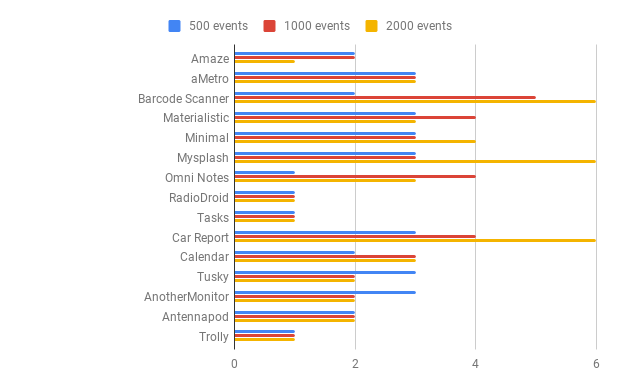
\includegraphics[width=0.9\textwidth]{img/monkeyNative.png}
	\caption{Number of discovered activities by Monkey executions with 500, 1,000 and 2,000 events over native applications}
	
	\label{monkeyNative}
\end{figure} 

%\begin{table*}[h]
%	\centering
%	\caption{Results of Wilcoxon signed ranks test for the number of activities found in native applications of Monkey executions ranging the number of events} \MARIO{why 5 and 6 samples? There should be 15 data per series (one datum per app)}
%	\label{WilcoxonMonkey}
%	\begin{adjustbox}{width=0.7\textwidth}
%		\begin{tabular}{|c|c|c|c|c|}
%			\hline
%			\textbf{Relation of events}&\textbf{500 - 1,000} & \textbf{500 - 2,000} & \textbf{1,000 - 2,000} \\\hline
%			\textbf{n samples}& 5 & 6 & 6 \\\hline
%			\textbf{Significance}& 10\% & 10\% & 10\% \\\hline
%			\textbf{T obtained value}& 1 & 3 & 3 \\\hline
%			\textbf{T critical value}& 0 & 2 & 2 \\\hline
%			\textbf{Diference?}& No & No & No \\\hline

%		\end{tabular}
%	\end{adjustbox}
%\end{table*}

\textbf{Hybrid applications.} Even though Monkey does not advertise special capabilities for hybrid applications, it was able to execute random events in the user interface. During the tests execution, it was evident that these random interactions made changes in the interface. Monkey is not designed to perform contextual changes in the application, however, due to the randomness of the GUI changes, in some rare cases it turned off or on airplane mode and connectivity settings.

Figure \ref{monkeyHybrid} Presents the discovered activities by Monkey with 500, 1000 and 2000 events. What this graph shows, is that almost for every app, the number of discovered activities was the same: 1. The explanation of this behavior comes from the conception of the hybrid app, with a single activity with a web view. The applications that contains more than a single activity are special cases that have multiple web views in different activities.

This experiment shows that even though Monkey made changes in the application, it only considers new activities as new states, it does not have a states memory. Monkey was successful interacting with the app, however, for hybrid apps, there is no way to determine how many states it visited if is not complemented with additional software.

\begin{figure}[t]
	\centering
	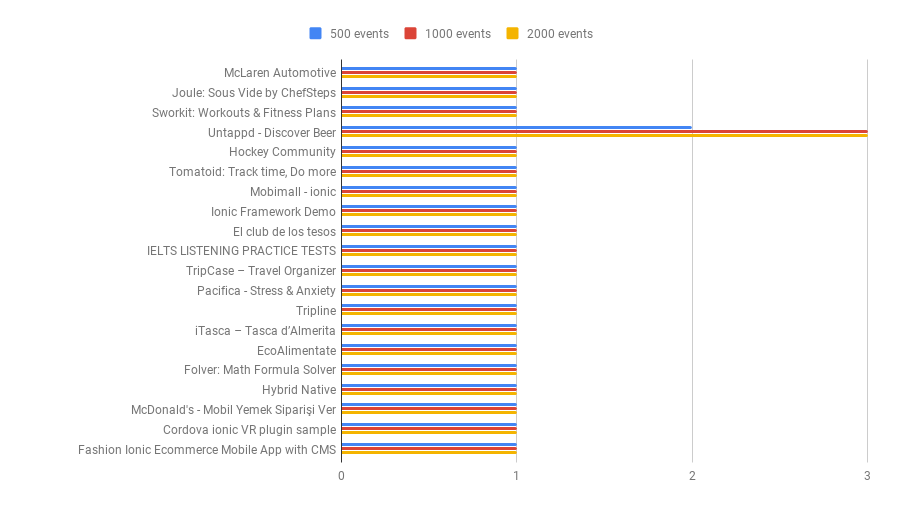
\includegraphics[width=0.9\textwidth]{img/monkeyHybrid.png}
	\caption{Number of discovered activities by Monkey executions with 500, 1,000 and 2,000 events over hybrid applications}
	
	\label{monkeyHybrid}
\end{figure} 

\textbf{Summary for UI/Application Exerciser Monkey.} The experiments show that Monkey is capable of identify different activities in native applications. However, changing the number of events performed does not make a significant difference in the number of activities encountered. Also, the average activity coverage of Monkey is 38\% in native applications, which suggests that a completely random discovery approach could be improved by a model-based approach.

As for hybrid applications, Monkey is not capable of reporting the number of states discovered insomuch as it only report activities. Monkey lacks ripping capabilities and does not aggregate results, which make analysis of its execution a hard task; a developer must follow all the events and activities to determine the states discovered by this random tool.

Based on the experiments conducted with this tool, we determined the importance of trigger random events in hybrid applications. This is a qualitative conclusion and tests to analyze quantitatively the importance of randomness in hybrid applications is part of our future work.

\subsection{Firebase Test Lab Robo Test}

Firebase Test Lab \cite{firebase} is one of the industry leaders in mobile testing. It has a cloud-based app-testing infrastructure that enables concurrent execution of tests with and without instrumentation. Firebase Test Lab Robo Test is one of their services: `Robo test analyzes the structure of your app's UI and then explores it methodically, automatically simulating user activities' \cite{firebase}. It cloud service allows testers to run Robo test on virtual and physical devices in parallel, detecting crashes and performance issues.

Firebase Test Lab was chosen in the study because it is the Google's flagship product in automated testing.

For each application, a Robo Test was configured and run. To configure each test, the developer must choose the specific device: in our case, \textit{Google Pixel's 2 API 27} was selected. The test recorded the number of actions performed during the exploration, the number of activities covered, the number of distinct screens visited and the duration. Is worth remembering that Firebase Test Lab is a cloud service and all the infrastructure is managed by Google. To that end, this service is very easy to use and the only requirement for the final user is to have the APK that he wants to test.

\textbf{Native applications.} The native applications were submitted to the service, and after each execution finished, Google sent an email informing the final result for every test. \tabref{FirebaseNative} presents the results of running Firebase Test Lab, indicating the duration, number of actions, activities and screens for the applications.  
\begin{table*}[t]
	\centering
	\caption{Results of running Firebase Test Lab on native applications}
	\label{FirebaseNative}
	\begin{adjustbox}{width=0.8\textwidth}
		\begin{tabular}{|c|c|c|c|c|}
			\hline
			\textbf{Application} & \textbf{Duration (s)} & \textbf{Actions} & \textbf{Activities} & \textbf{Screens} \\\hline
			Amaze & 314 & 268 & 1 & 120 \\\hline
			aMetro & 309 & 343 & 4 & 73 \\\hline
			Barcode Scanner & 258 & 204 & 7 & 27 \\\hline
			Materialistic & 301 & 87 & 6 & 28 \\\hline
			Minimal & 304 & 200 & 4 & 26 \\\hline
			Mysplash & 313 & 68 & 6 & 23 \\\hline
			Omni Notes & 25 & 8 & 1 & 3 \\\hline
			RadioDroid & 313 & 122 & 1 & 79 \\\hline
			Tasks & 303 & 227 & 6 & 90 \\\hline
			Car Report & 305 & 202 & 5 & 37 \\\hline
			Calendar & 304 & 205 & 6 & 64 \\\hline
			Tusky & 33 & 12 & 1 & 4 \\\hline
			AnotherMonitor & 318 & 133 & 4 & 19 \\\hline
			Antennapod & 314 & 141 & 5 & 59 \\\hline
			Trolly & 11 & 7 & 1 & 1 \\\hline
		\end{tabular}
	\end{adjustbox}
\end{table*}
Figure \ref{firebase} depicts the outcomes of the execution for a specific app, including a full video of the whole crawling process, aggregated statistics and a very detailed crawl graph. This graph shows the different screens connected with edges associated to clicks and button pressings. The applications that seem to have a low number of screens (\eg Trolly: 1, Omni Notes: 3) have login and authentication activities in the applications. In these scenarios, Testlab is unable to automatically create users or introduce credentials, and does not explore more than the initial screens. 

\begin{figure}[t]
	\centering
	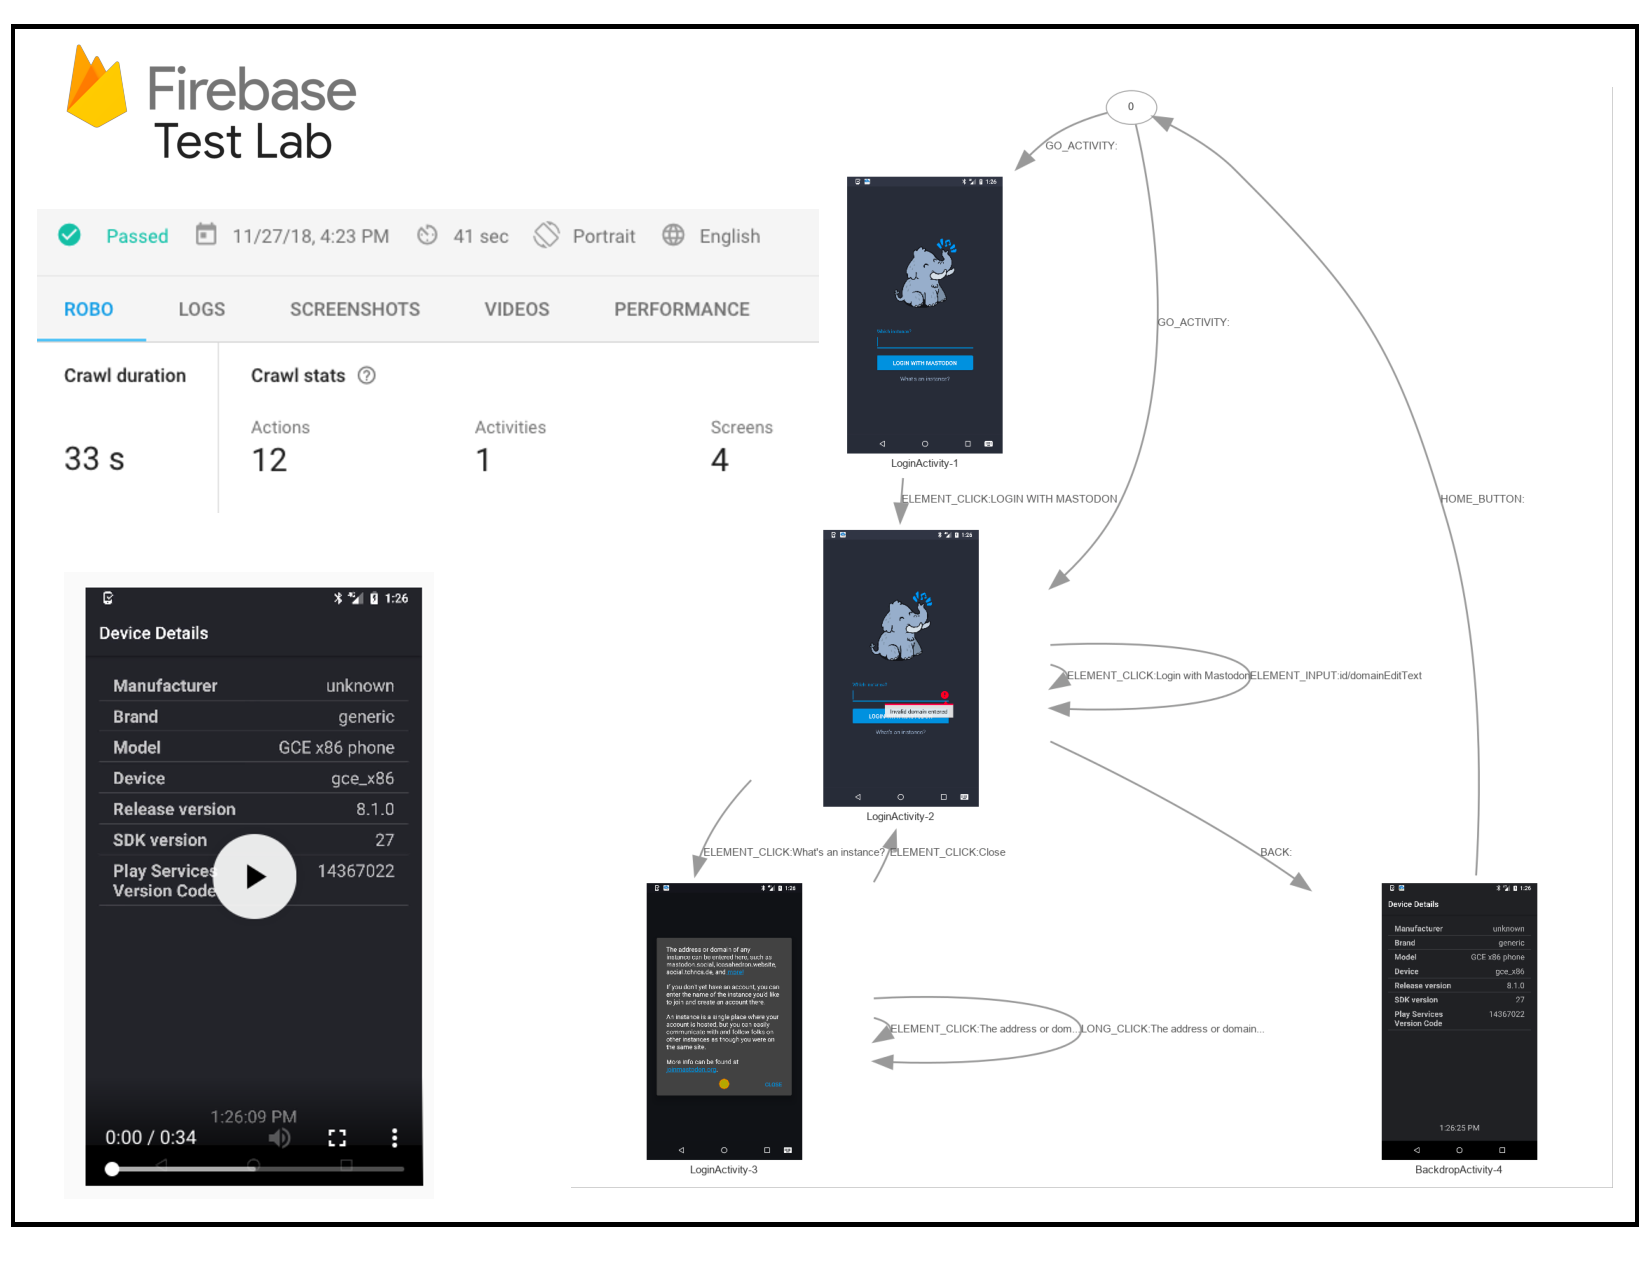
\includegraphics[width=1\textwidth]{img/firebase.pdf}
	\caption{Firebase Test Lab: Results of a Robo Test for a single native app}
	
	\label{firebase}
\end{figure} 

\textbf{Hybrid applications.} Regarding hybrid applications, Firebase Test Lab's behavior was entirely different from its native execution \tabref{FirebaseHybrid}. In almost all the applications, the number of activities discovered was 1 because hybrid apps usually do not have more than one activity. There are two groups of apps: those with a number of screens greater than 60 and those with a number of screens lower than 10. Examining carefully those applications with a big number of screens found, we identified that Firebase classified screens with animations as multiple screens; one of this cases is presented in Figure \ref{multipleScreens}.  In this figure, an animation is running in the background of the screen, the animation is continuously changing. The Robo Test is visually detecting updates in the screen, and as the frames change, it detects new screens of the application.

\textbf{Summary of Firebase Test Lab Robo Test.} Firebase Test Lab is a easy to use service that explored native and hybrid applications in a short time. It detected several different screen in hybrid applications, however, it did not explore correctly hybrid applications. In none of them it was able to detect the states correctly and build the crawl graph.

\begin{table*}[t]
\centering
\caption{Results of running Firebase Test Lab on hybrid applications}
\label{FirebaseHybrid}
\begin{adjustbox}{width=0.9\textwidth}
	\begin{tabular}{|c|c|c|c|c|}
		\hline
		\textbf{Application} & \textbf{Duration (s)} & \textbf{Actions} & \textbf{Activities} & \textbf{Screens} \\\hline
		McLaren Automotive & 15 & 4 & 1 & 3 \\\hline
		Joule & 306 & 194 & 1 & 146 \\\hline
		Sworkit & 163 & 63 & 1 & 6 \\\hline
		Untappd & 9 & 6 & 1 & 2 \\\hline
		Hockey Community & 322 & 20 & 1 & 3 \\\hline
		Tomatoid & 86 & 70 & 1 & 3 \\\hline
		Mobimall & 9 & 8 & 1 & 2 \\\hline
		Ionic Framework & 37 & 10 & 1 & 3 \\\hline
		El club de los tesos & 11 & 4 & 1 & 3 \\\hline
		IELTS PRACTICE & 253 & 79 & 2 & 5 \\\hline
		TripCase & 26 & 15 & 1 & 3 \\\hline
		Pacifica & 282 & 235 & 4 & 62 \\\hline
		Tripline & 82 & 24 & 1 & 4 \\\hline
		iTasca & 79 & 17 & 1 & 3 \\\hline
		EcoAlimentate & 5 & 4 & 1 & 2 \\\hline
		Folver & 74 & 22 & 1 & 6 \\\hline
		Hybrid Native & 144 & 31 & 2 & 9 \\\hline
		McDonald's & 91 & 28 & 1 & 3 \\\hline
		Cordova ionic VR & 80 & 21 & 2 & 9 \\\hline
		Fashion Ecommerce & 72 & 17 & 1 & 2 \\\hline
	\end{tabular}
\end{adjustbox}
\end{table*}
% \begin{figure}[t]
%	\centering
%	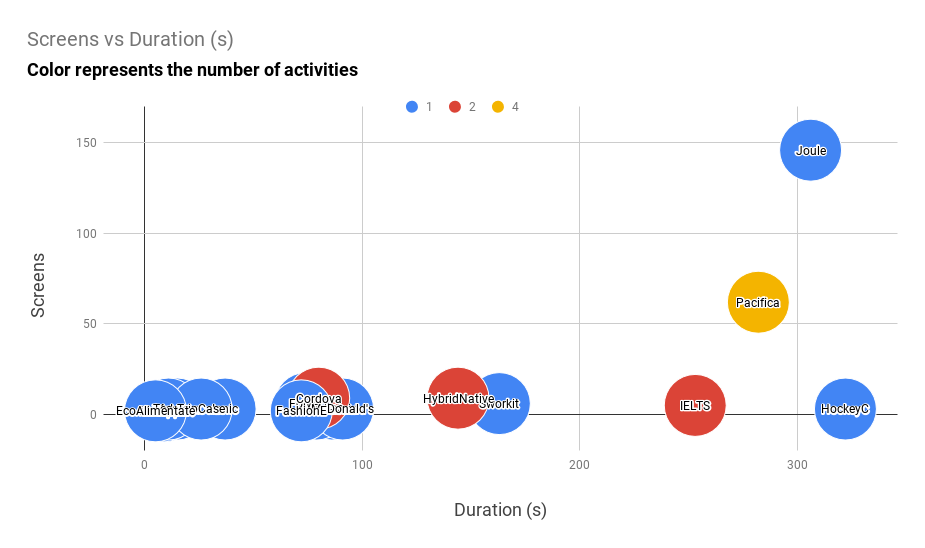
\includegraphics[width=1\textwidth]{img/screensVsDurationFhybrid.png}
%	\caption{Firebase: Number of screens vs duration\textit{ Color represents the number of detected activities}}	
%	\label{screensVsDurationFhybrid}
%\end{figure} 
\begin{figure}[t]
	\centering
	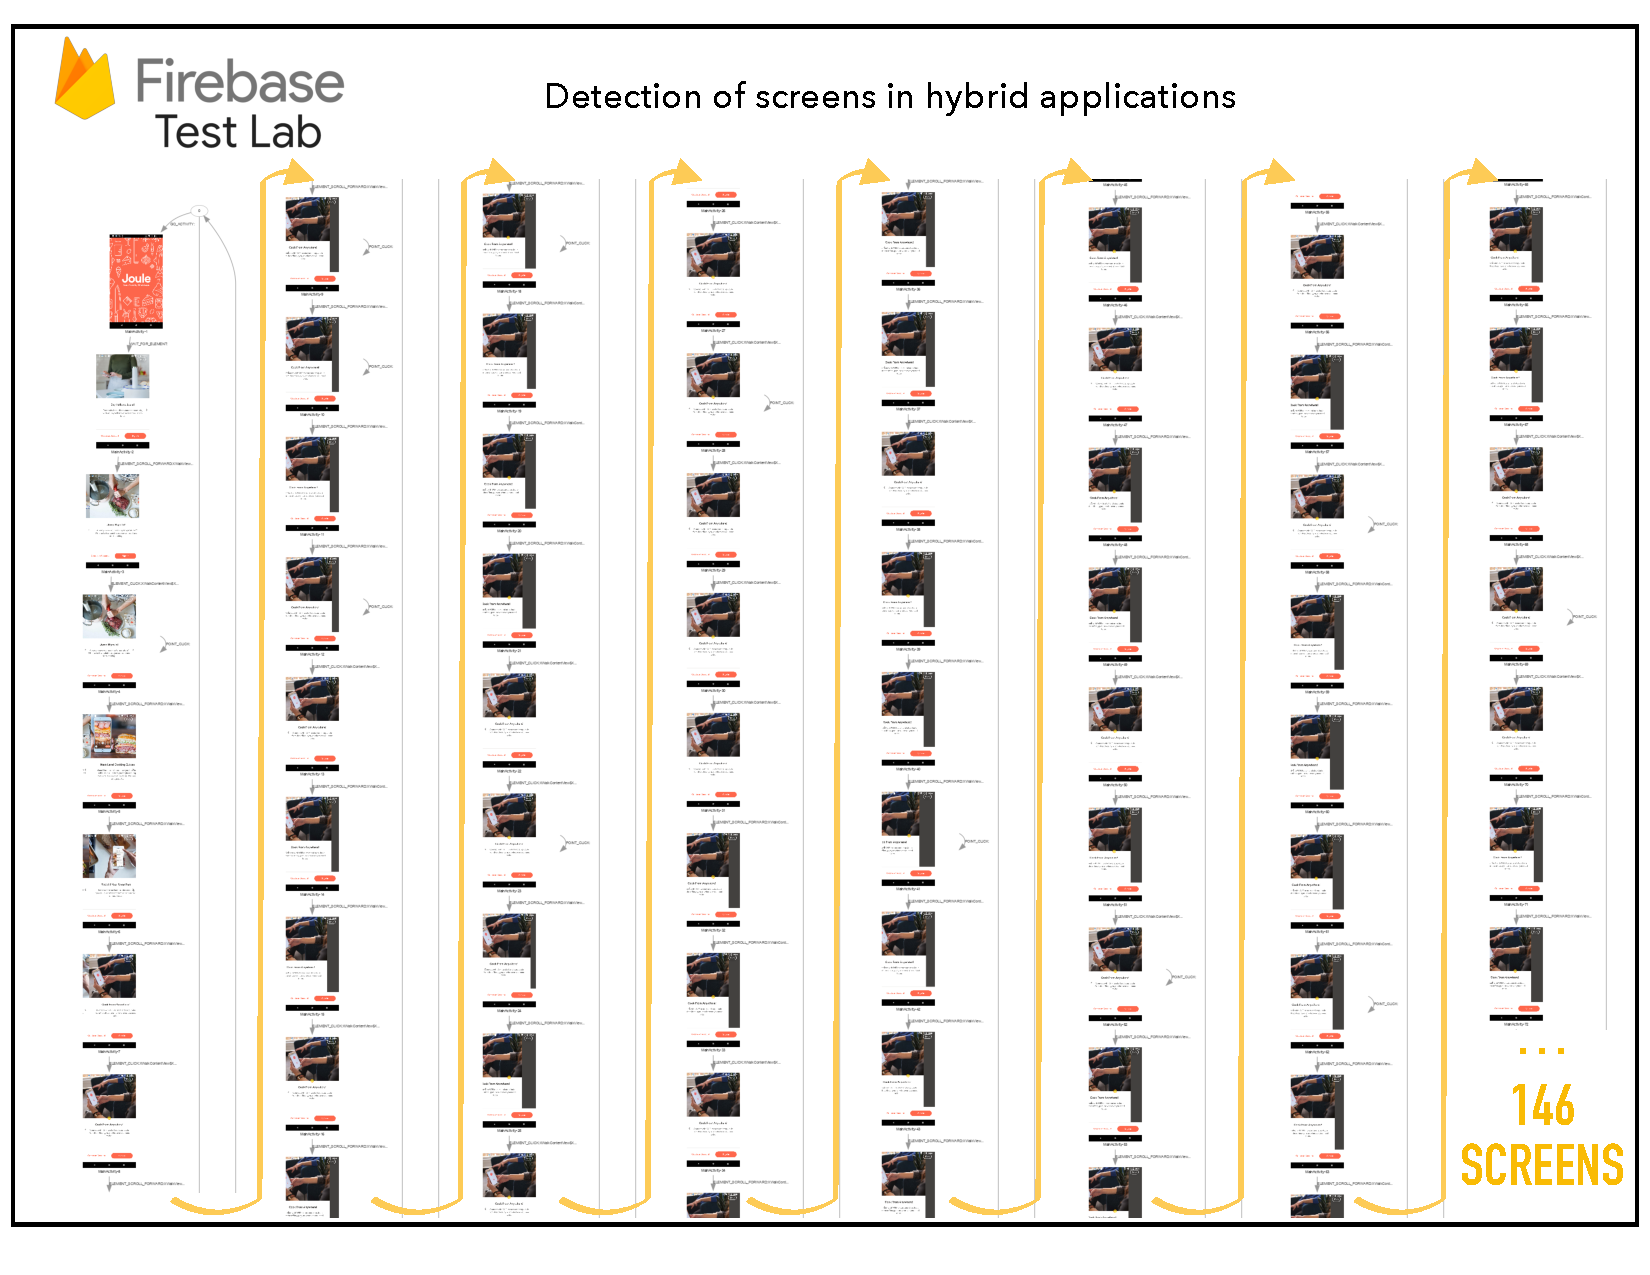
\includegraphics[width=1\textwidth]{img/multipleScreens.pdf}
	\vspace{-0.8cm}
	\caption{For some hybrid apps with animations, Firebase detect the same state multiple times and reports a unreal number of screens}
	
	\label{multipleScreens}
\end{figure} 



\subsection{DroidBot}

DroidBot \cite{Li:ICSE17} is a tool that uses a model-based strategy to automatically explore mobile GUIs. It generates inputs and a transition model between different states of the application. One of the main features of DroidBot is that it does not require app instrumentation and is mean to run in almost any Android device. DroidBot is open source and publicly available \cite{droidbotRepo}.
It was choose as a baseline for the study because its availability and effectiveness exploring mobile applications.

DroidBot was executed running the command \texttt{droidbot <APK name> -o <Output folder> -is\_emulator -random} for the complete set of applications. The \texttt{-random}  flas was used to add randomness to input events and the \texttt{-is\_emulator}  flag was required for running droidbot on virtual devices . The exploration strategy used was \textit{dfs\_greedy} which explores UI using a greedy depth-first strategy. DroidBot implements other search strategies (\eg \textit{dfs\_naive}, \textit{bfs\_naive}, \textit{bfs\_greedy}), but  \textit{dfs\_greedy} was chosen because this strategy is a better approximation when trying to explore completely a tree.

For each tested application DroidBot generates a UTG (\textit{UI Transition Graph}), screen shots of the states and an HTML report that includes the time spent, number of input events, number of UTG states, number of UTG edges and activity coverage.

\textbf{Native applications.} The results of DroidBot on native applications are shown in \tabref{DroidNative}, the average activity coverage is 52\% and  the average duration is 73 minutes. Also, the number of input events rounds 990 and the discovered states range between 37 and 874 with a standard deviation of 218. It can be seen that the average duration of the test is more than 10 times the maximum duration of a Robo test in Firebase. Also, from the state graphs generated it can be noticed that many of the states registered by DroidBot are almost the same, they share the same layout but only the content in the fields changes. For example, the most repeated case is in a login form, each time DroidBot changes the input fields a state is reported. Moreover, if DroidBot leaves the login view and comes back after, it reports again all the states generated from login view.

\begin{table*}[t]
	\centering
	\caption{Results of running DroidBot  on native applications  \textbf{Abbreviations for column headings}. \textit{RA} = Registered activities in the app, \textit{FA} = Found activities during exploration, \textit{AC} = Activity coverage, \textit{Time(s)} = Time of execution, Input events = Number of input events generated, \textit{UTG states} = UI Transition Graph States, \textit{UTG edges} = UI Transition graph edges}
	\label{DroidNative}
	\begin{adjustbox}{width=\textwidth}
		\begin{tabular}{|c|c|c|c|c|c|c|c|}
			\hline
			\textbf{App} & \textbf{RA} & \textbf{FA} & \textbf{AC} & \textbf{Time(s)} & \textbf{Input events} & \textbf{UTG states} & \textbf{UTG edges} \\\hline
			Amaze & 6 & 2 & 0.33 & 4492 & 996 & 295 & 453 \\\hline
			aMetro & 6 & 4 & 0.66 & 3966 & 998 & 108 & 248 \\\hline
			Barcode Scanner & 9 & 7 & 0.77 & 4173 & 997 & 49 & 106 \\\hline
			Material Notes & 23 & 6 & 0.26 & 5944 & 990 & 120 & 345 \\\hline
			Minimal & 5 & 4 & 0.8 & 3756 & 997 & 150 & 342 \\\hline
			Mysplash & 20 & 7 & 0.35 & 6796 & 995 & 221 & 489 \\\hline
			Omni Notes & 17 & 4 & 0.23 & 4238 & 992 & 196 & 405\\\hline
			RadioDroid & 2 & 1 & 0.5 & 3959 & 990 & 453 & 548\\\hline
			Tasks & 38 & 5 & 0.13 & 3437 & 997 & 69 & 116\\\hline
			Car Report & 8 & 7 & 0.87 & 4607 & 997 & 254 & 402 \\\hline
			Calendar & 12 & 7 & 0.58 & 4068 & 996 & 227 & 313\\\hline
			Tusky & 21 & 1 & 0.04 & 4754 & 996 & 16 & 37 \\\hline
			AnotherMonitor & 4 & 4 & 1 & 3437 & 995 & 819 & 874\\\hline
			Antennapod & 20 & 7 & 0.35 & 4434 & 997 & 328 & 518\\\hline
			Trolly & 2 & 2 & 1 & 3745 & 992 & 35 & 89 \\\hline
		\end{tabular}
	\end{adjustbox}
\end{table*}

\textbf{Hybrid applications.} The results of running DroidBot on hybrid applications are shown in \tabref{DroidHybrid}, it can be noticed that even though there are multiple registered activities in most of the applications, only one is discovered by the tool. This is due to the fact that the hybrid applications use a Web View which encapsulates the GUI components using, in most of the cases, only one activity.

Moreover, the average duration of the test was 68 minutes, the number of input events ranges between 723 and 998, and the average number of discovered states is 94.1. However, from the state graphs it can be seen that as DroidBot is unable to analyze the Web View, it keeps exploring outer applications like Facebook or Google (accessing to these services in the authentication screen). Also, DroidBot does not report only different states, we manually counted the number of repeated and outer application states and reported them as false positives. It was estimated that the 67.1\% of the states discovered correspond to false positives. As can be seen in Figure \ref{repeated}, extracted from a state graph generated by DroidBot, there are several states reported that share the same view.

\begin{figure}[t]
	\centering
	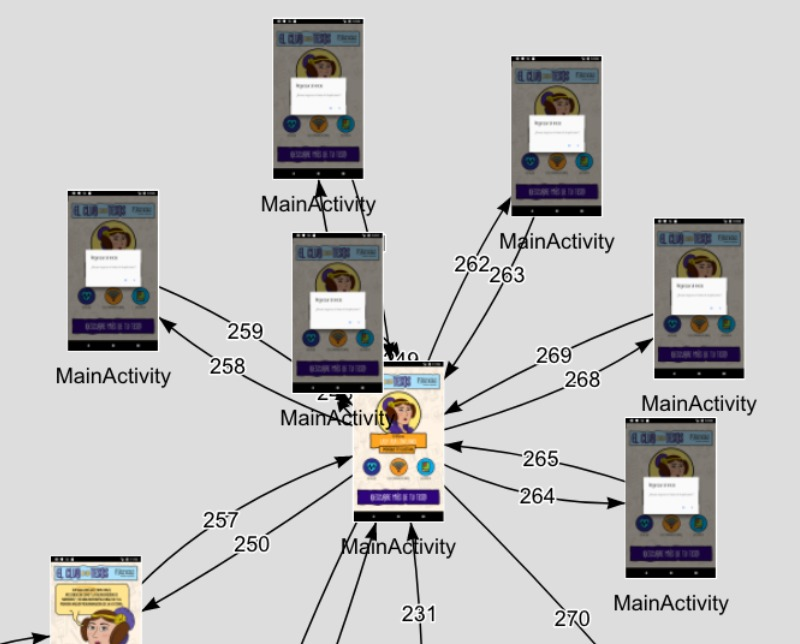
\includegraphics[width=0.8\textwidth]{img/exRepeated.png}
	\caption{Example of repeated states discovered by DroidBot}
	
	\label{repeated}
\end{figure} 

\begin{table*}[h]
	\centering
	\caption{Results of running DroidBot  on hybrid applications  \textbf{Abbreviations for column headings}. \textit{RA} = Registered activities in the app, \textit{FA} = Found activities during exploration, \textit{AC} = Activity coverage, \textit{Time(s)} = Time of execution, Input events = Number of input events generated, \textit{UTG states} = UI Transition Graph States, \textit{UTG edges} = UI Transition graph edges, \textit{FP States} = False positive states discovered.}
	\label{DroidHybrid}
	\begin{adjustbox}{width=\textwidth}
		\begin{tabular}{|c|c|c|c|c|c|c|c|c|}
			\hline
			\textbf{App} & \textbf{RA} & \textbf{FA} & \textbf{AC} & \textbf{Time(s)} & \textbf{Input events} & \textbf{UTG states} & \textbf{UTG edges} & \textbf{FP States}\\\hline
			McLaren Automotive & 6 & 1 & 0.16 & 3042 & 723 & 70 & 127 & 50 \\\hline
			Joule & 8 & 1 & 0.12 & 4792 & 997 & 65 & 120 & 49 \\\hline
			Sworkit & 14 & 2 & 0.14 & 8270 & 996 & 87 & 200 & 65 \\\hline
			Untappd & 11 & 2 & 0.18 & 3849 & 997 & 76 & 154 & 32 \\\hline
			Hockey Community & 17 & 2 & 0.11 & 3652 & 996 & 143 & 360 & 129 \\\hline
			Tomatoid & 1 & 1 & 1 & 3835 & 989 & 112 & 183 & 80 \\\hline
			Mobimall & 12 & 1 & 0.08 & 3508 & 997 & 174 & 388 & 155\\\hline
			Ionic Framework & 1 & 1 & 1 & 3410 & 997 & 256 & 558 & 254\\\hline
			El club de los tesos & 1 & 1 & 1 & 4035 & 997 & 32 & 99 & 14\\\hline
			IELTS PRACTICE & 2 & 2 & 1 & 3782 & 998 & 86 & 229 & 79\\\hline
			TripCase & 14 & 2 & 0.14 & 4072 & 992 & 142 & 240 & 122\\\hline
			Pacifica & 10 & 2 & 0.2 & 4005 & 993 & 116 & 301 & 107\\\hline
			Tripline & 3 & 1 & 0.33 & 3953 & 997 & 59 & 175 & 39\\\hline
			iTasca & 1 & 1 & 1 & 4179 & 997 & 61 & 129 & 49\\\hline
			EcoAlimentate & 1 & 1 & 1 & 3733 & 997 & 8 & 19 & 4\\\hline
			Folver & 4 & 1 & 0.25 & 3654 & 997 & 32 & 93 & 15\\\hline
			Hybrid Native & 1 & 1 & 1 & 3383 & 989 & 36 & 78 & 22\\\hline
			McDonald's & 5 & 1 & 0.2 & 4012 & 997 & 28 & 63 & 10\\\hline
			Cordova ionic VR & 3 & 1 & 0.33 & 3573 & 997 & 289 & 593 & 219\\\hline
			Fashion Ecommerce & 18 & 1 & 0.05 & 5105 & 997 & 10 & 19 & 0\\\hline
		\end{tabular}
	\end{adjustbox}
\end{table*}

\textbf{Summary for DroidBot.} DroidBot is able to generate a state graph from the ripping, it also reports the number of states discovered and its transitions. In native applications, it obtains an average activity coverage of 52\% on native applications, which is higher to the obtained by Firebase (44\%) and Monkey (38\%). However, the time spent in the test is more than 10 times the maximum duration of a Robo test in Firebase, this opens the possibility to find new approaches of ripping that increase the activity coverage in less time.  

As for hybrid applications, DroidBot is unable to analyze the Web View; therefore, it runs out of the main application generating a lot of states that does not refer to the application under test, and does not report the number of different states generating a large number of false positive states (67.1\%). 
\subsection{RIP}
We also analyzed the apps with our proposed tool, \textbf{RIP}.
 
\textbf{Native applications.} In order to compare RIP with Firebase and DroidBot, Table \ref{comparisonRIP} presents the average activity coverage, average number of states discovered, standard deviation of the number of states discovered, the average duration of the tests and the average number of new states discovered when applying contextual changes. It can be noticed that the higher activity coverage is reached by DroidBot (50.15\%) however, its average duration is about 17 times higher than Firebase and 14 times higher than RIP. The average number of states found by DroidBot is 5 times higher than Firebase and 7 times higher than RIP. 
Nevertheless, neither DroidBot nor Firebase apply contextual changes in the exploration of states. With contextual changes RIP reported 6.33 new states discovered on average.

RIP exploration algorithm was behind Firebase and DroidBot, however, enabling contextual changes in exploration allows \textbf{RIP} to find states that these tools are not able to detect.

Monkey was not included in this comparison because Monkey only reports different activities reached and does not rip the applications, it only triggers random events during the execution, and records in a log the activities found and the events triggered. From monkey's execution, it was valuable to see that its random approach sometimes toggle rare settings, that were hardly discovered from systematic approaches. This random exploration is very useful to detect crashes, however, is not  useful  at all for building a multi-model because it is difficulty to reproduce large and unguided scenarios generated by Monkey.

\begin{table*}[t]
	\centering
	\caption{Comparison in native applications between RIP, DroidBot and Firebase. \textbf{Abbreviations for row headings}. \textit{Std states} = Standard deviation of the number of states discovered,  \textit{\# States CC} = Number of states discovered when applying contextual changes. }
	\label{comparisonRIP}
	\begin{adjustbox}{width=0.6\textwidth}
		\begin{tabular}{|c|c|c|c|c|}
			\hline
			\textbf{Average metric}&\textbf{RIP} & \textbf{DroidBot} & \textbf{Firebase} \\\hline
			\textbf{Activity coverage}& 34.97\% & 50.15\% & 44.07\% \\\hline
			\textbf{\# States}& 28.06 & 222.66 & 43.53 \\\hline
			\textbf{Std states}& 24.63 & 204.83 & 35.55 \\\hline
			\textbf{Duration (min)}& 4.93 & 73.11 & 4.13 \\\hline
			\textbf{\# States CC}& 6.33 & - & - \\\hline
			
		\end{tabular}
	\end{adjustbox}
\end{table*}


\textbf{Hybrid applications.} In order to compare the state discovery algorithm implemented in RIP with Firebase and DroidBot (true positives only), we recorded the number of states discovered by each tool.  As it can be seen in Figure \ref{ripRad}, RIP detects a larger number of states almost in all applications compared to DroidBot and Firebase. 

It can be observed from \tabref{comparisonRIPHybrid} that the average number of true positive states discovered by RIP is 50.1, without outer applications or repeated states. Also, the average duration of RIP was 7.31 minutes which is 10 times less than the average duration of DroidBot. The number of states discovered by Firebase is 3 times lower than RIP's. Finally, in hybrid applications the only tool able to do contextual changes and detect new states generated is RIP, and it found in average 5.6 new states with this changes. 

The comparison of RIP vs Firebase performance is presented in Figure \ref{ripFirebase}. RIP was able to extract a complete graph from the hybrid application explored, including all the views and screens of the application. Firebase Test Lab opened the application, detected the splash view, and then the main screen of the application. After that, Firebase was unable to detect the components of the application. Related to hybrid apps exploration, RIP is superior.


\begin{figure}[t]
	\centering
	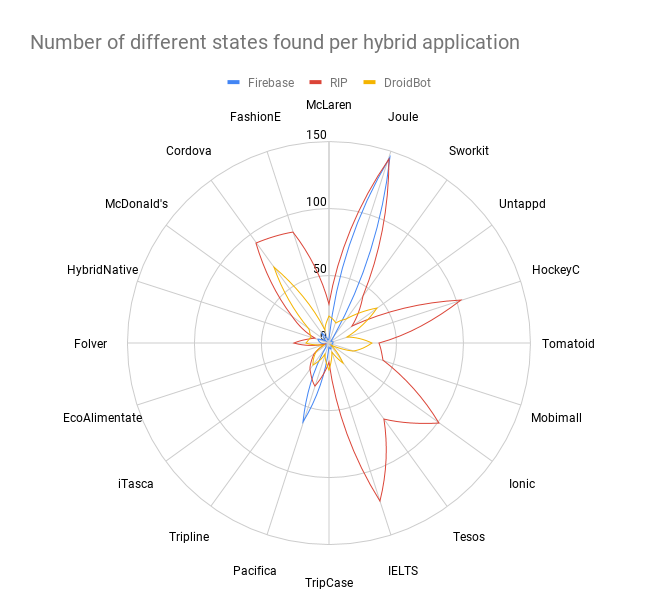
\includegraphics[width=1.1\textwidth]{img/ripRadComp.png}
	\vspace{-0.8cm}
	\caption{Comparison of the number of different states discovered on hybrid applications between RIP, Firebase and DroidBot}
	
	\label{ripRad}
\end{figure} 

\begin{table*}[t]
	\centering
	\caption{Comparison in hybrid applications between RIP, DroidBot and Firebase. \textbf{Abbreviations for row headings}. \textit{Std states} = Standard deviation of the number of states discovered,  \textit{\# States CC} = Number of states discovered when applying contextual changes, \textit{ \# TP states} = Number of different states discovered, \textit{FP states percentage} = Percentage of repeated or outer application or repeated states discovered. }
	\label{comparisonRIPHybrid}
	\begin{adjustbox}{width=0.6\textwidth}
		\begin{tabular}{|c|c|c|c|c|}
			\hline
			\textbf{Average metric}&\textbf{RIP} & \textbf{DroidBot} & \textbf{Firebase} \\\hline
			\textbf{\# States}& 52.6 & 94.1 & 13.95 \\\hline
			\textbf{Std states}& 39.29 & 76.16 & 33.74 \\\hline
			\textbf{\# TP States}& 50.1 & 19.4 & 12.7 \\\hline
			\textbf{Duration (min)}& 7.31 & 68.2 & 1.78 \\\hline
			\textbf{\# States CC}& 5.6 & - & - \\\hline
			\textbf{FP states percentage}& 4\% & 67.1\% & 5\% \\\hline
			
		\end{tabular}
	\end{adjustbox}
\end{table*}

\begin{figure}[t]
	\centering
	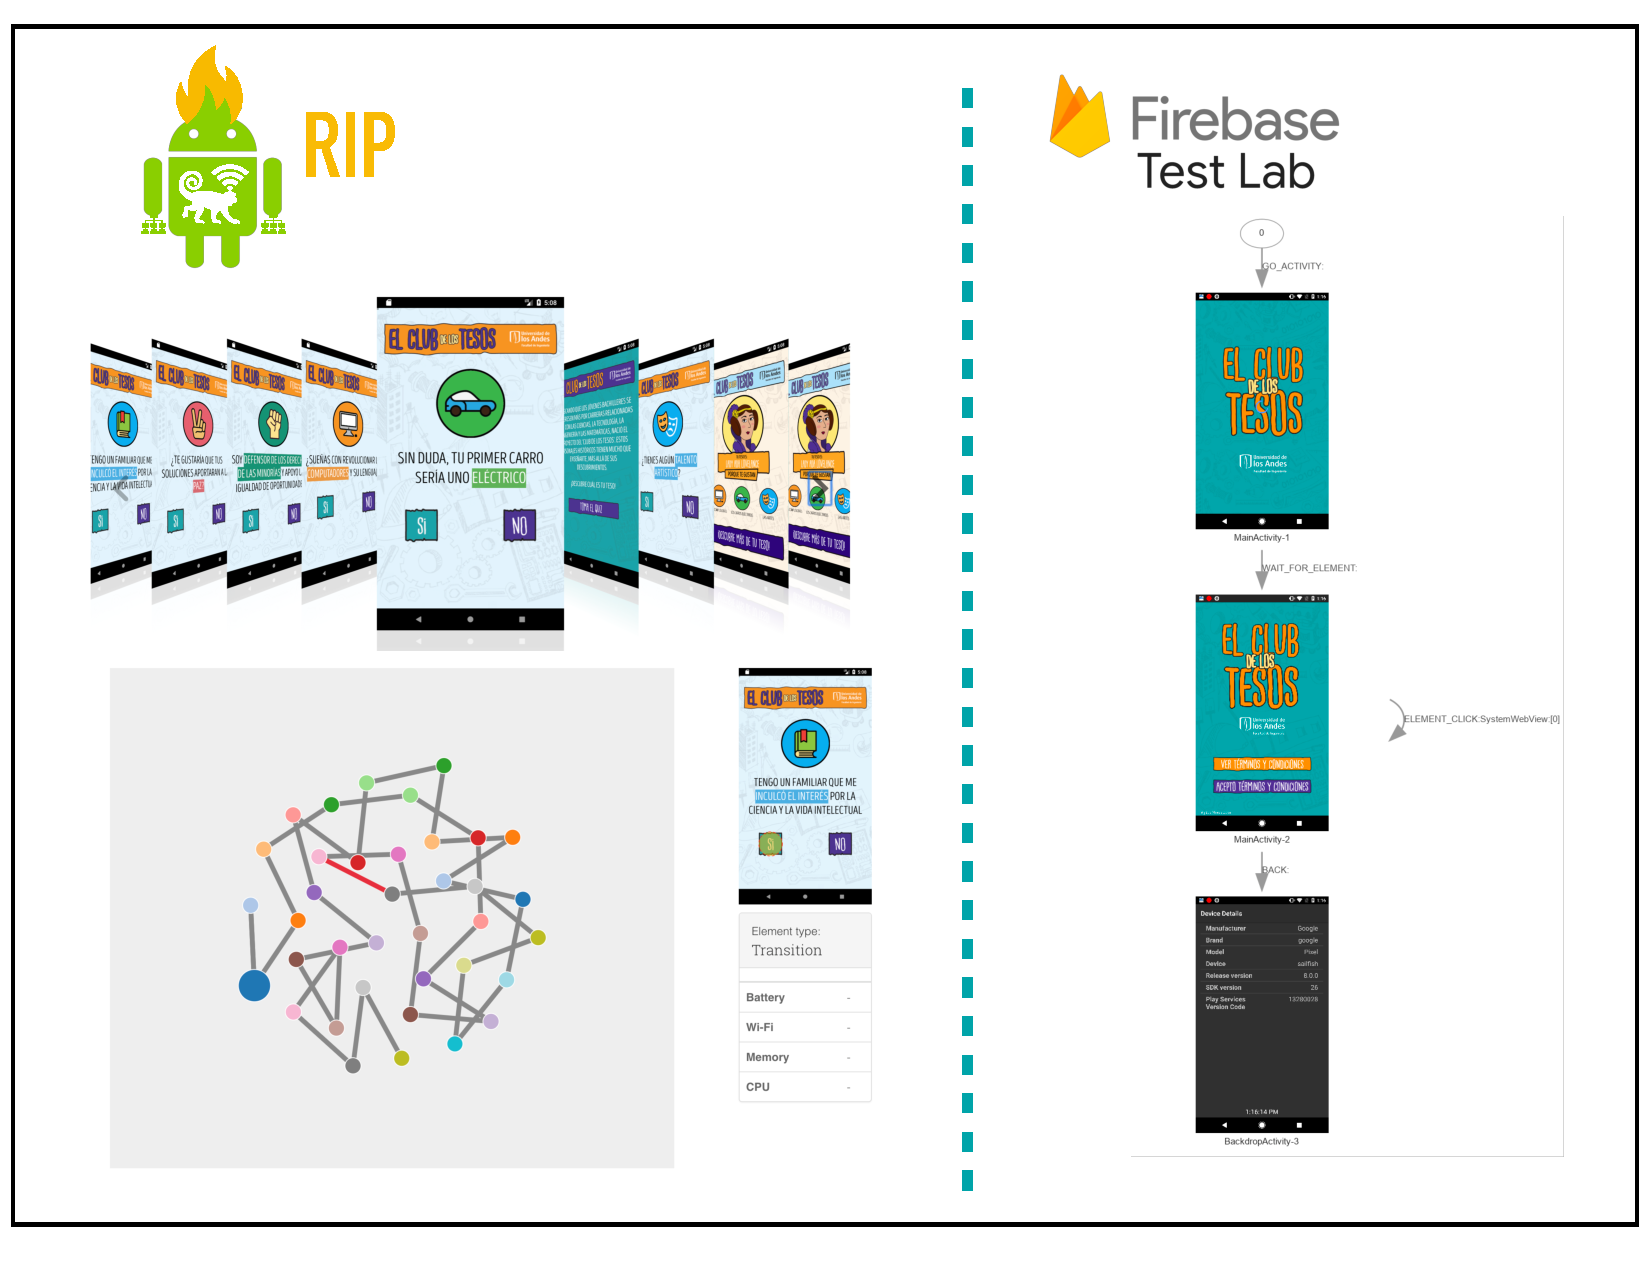
\includegraphics[width=1\textwidth]{img/ripFirebase.pdf}
	\vspace{-0.5cm}
	\caption{Comparison of a hybrid app exploration between RIP and Firebase Test Lab Robo. Firebase only found 2 states of the app: the main screen and the splash image}
	
	\label{ripFirebase}
\end{figure} 

\begin{tcolorbox}[title= \textit{\textbf{RQ$_2$}} How accurate is the \textit{state discovery algorithm} implemented in RIP when compared to state-of-the art tools?]
	Still performance of \textbf{RIP} exploring native applications is lower than existing baseline tools' (based only on GUI ripping), enabling contextual changes in exploration allows \textbf{RIP} to find states that these tools are not able to detect. 
	
	Our tool bridges the gap of ripping hybrid apps, and is the first approach that focuses in exploring dynamically these applications. \textbf{RIP} outperforms industry and academy state of the art tools in the exploration of hybrid apps in terms of detecting new states and not including repeated states in the crawl graph. 
\end{tcolorbox}

\section{\textbf{RQ$_3$} Is RIP suitable to detect crashes and bugs in Android apps?}

To answer \textit{\textbf{RQ$_3$}}, a third case study was carried out in parallel to the experiments of \textit{\textbf{RQ$_2$}}. While exploring each one of the applications, the number of crashes was obtained from \textbf{RIP}, Firebase and Monkey. Crashes from Monkey were extracted manually from the Monkey's log because it does not report aggregated results. In addition, DroidBot was not included in this case study because it neither report crashes nor bugs.

In the complete set of applications, Monkey found one crash in a native application. During the execution of Monkey in hybrid applications, it was able to triggered events that caused ANRs and HTTP errors, however, it was not able to register them because Monkey only detect native crashes.

In native apps, RIP found 2 crashes related to contextual changes (turning on airplane mode) These crashes occurred when the device was connected to Internet and lost connection while executing a background download task. In hybrid applications, RIP found a series of crashes which are presented in the Figure \ref{crashes}. It found crashes in 40 \% of the hybrid applications presented in the list. These crashes include HTTP 500 errors (Internal server errors without description), HTTP 503 errors (Service unavailable) and HTTP 404 errors (not found errors). Some of these crashes are depicted in Figure \ref{ripFindsCrashes}.

\begin{figure}[t]
	\centering
	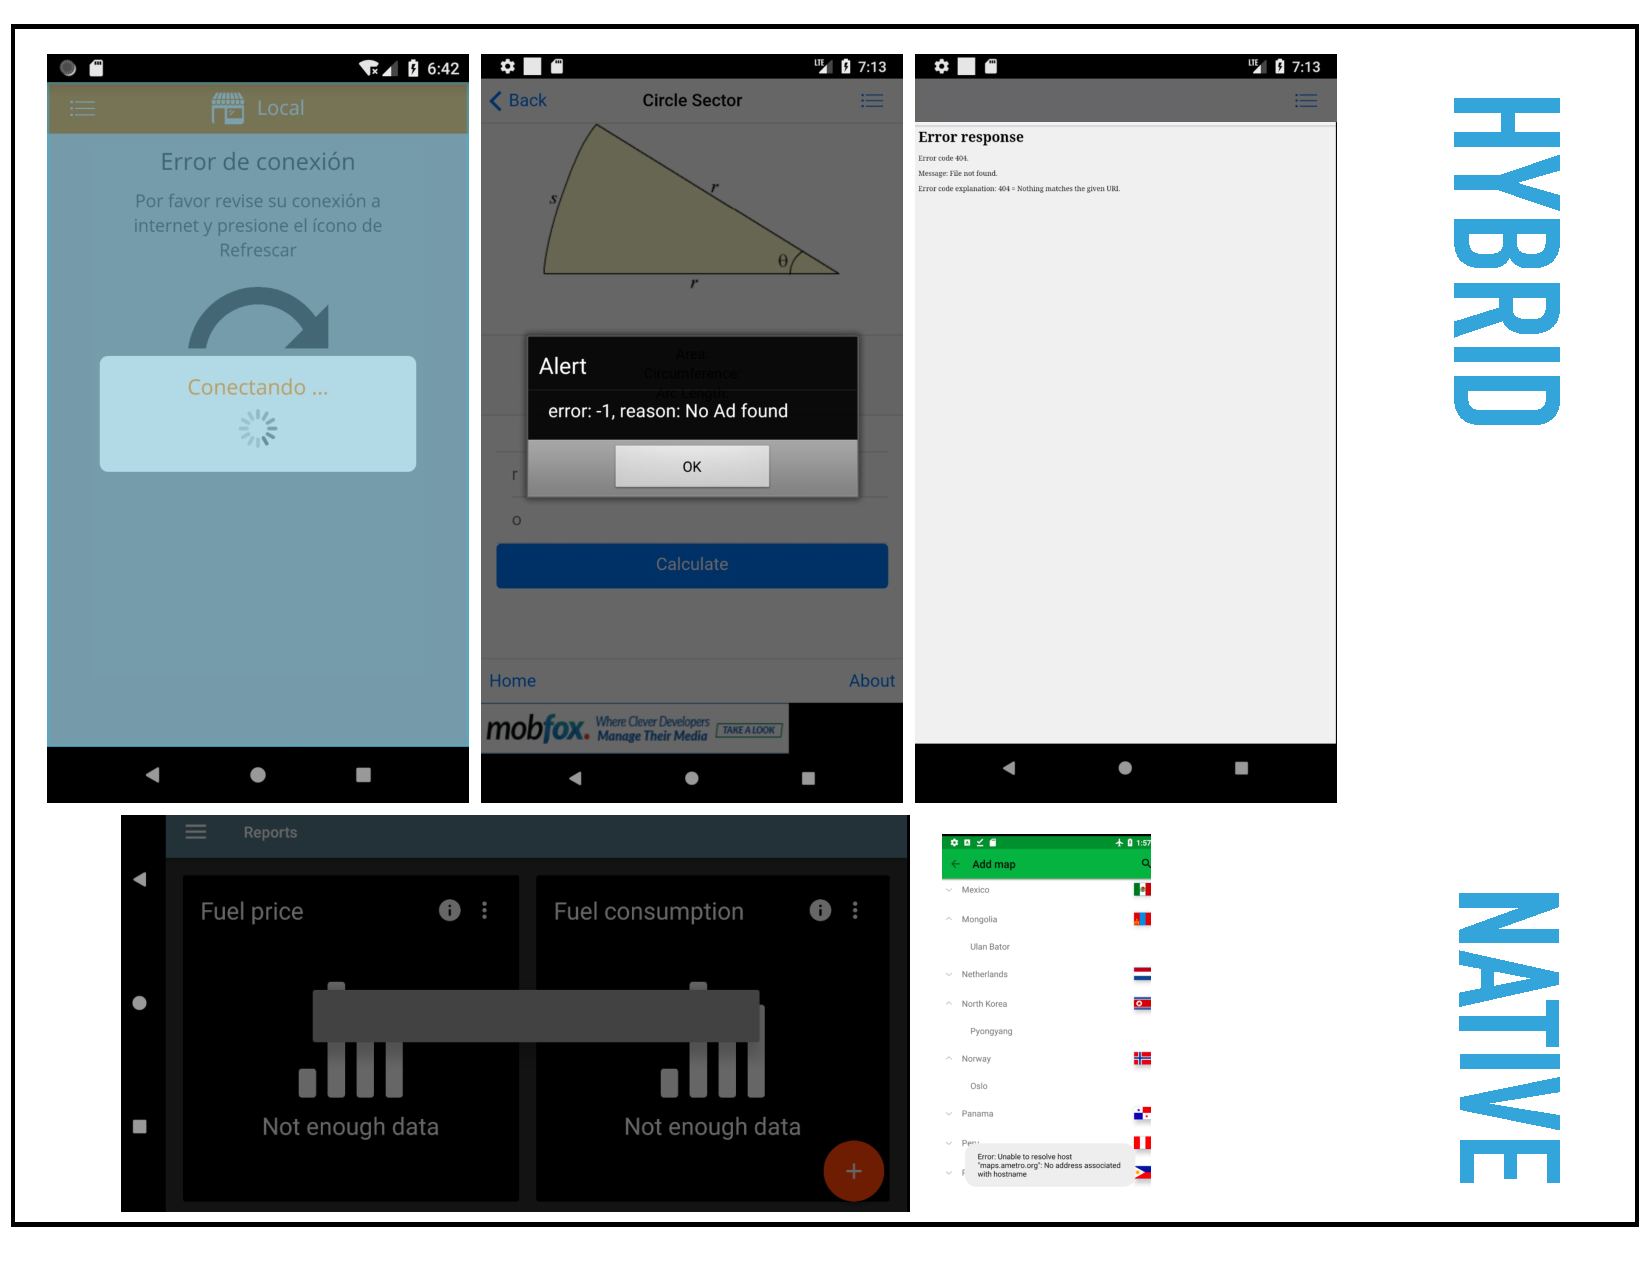
\includegraphics[width=1\textwidth]{img/errorHybrid.pdf}
	\vspace{-0.5cm}
	\caption{Crashes found by \textbf{RIP}}
	\label{ripFindsCrashes}
\end{figure} 


Firebase Test Lab was not able to find crashes in none of the hybrid applications, and did not discover the crashes in the native applications because they were triggered by contextual changes.

We realized that mobile hybrid applications require extensively external web information, and in most cases, the lack of connectivity in the device is not well managed. These scenarios were common, and caused the aforementioned errors.

\begin{figure}[t]
	\centering
	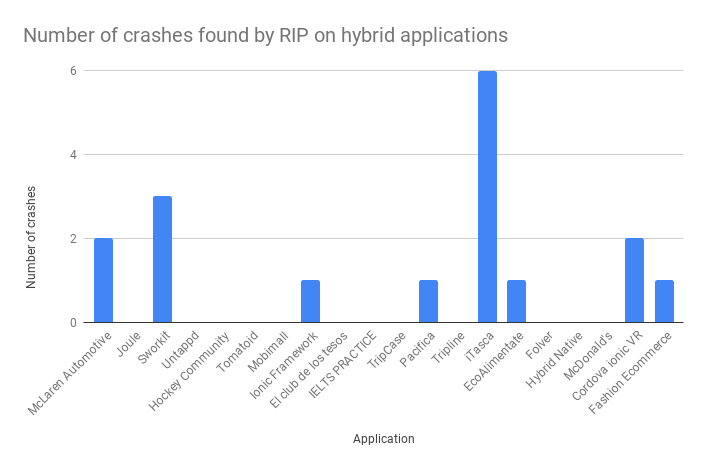
\includegraphics[width=1\textwidth]{img/crashes.png}
	\vspace{-0.5cm}
	\caption{Number of crashes identified by RIP for each hybrid application}.
	
	\label{crashes}
\end{figure} 

\begin{tcolorbox}[title= \textit{\textbf{RQ$_3$}} Is RIP suitable to detect crashes and bugs in Android apps?]
	\textbf{RIP} is able to detect WEB and HTTP crashes from hybrid applications based on the WebView Javascript console whereas native based tools only detect crashes such as \texttt{IOException} or \texttt{OutOfMemoryError}. RIP also detects native crashes reported by the system in the \texttt{logcat}. This combination of web information and native informations gives \textbf{RIP} and advantage over existing tools.
	
\end{tcolorbox}
 % INCLUDE: concepts
% !TEX root = ../thesis-example.tex
%
\chapter{Conclusion}
\label{chapter5}

The results from our empirical study suggest that  automatically extracting augmented models from Android apps enables better understanding of the apps. For modern mobile applications, ripping apps --- but based only on GUI exploration--- is not enough because they are context-aware. To that end, context, GUI, usage and domain models should be extracted and combined together to build more useful and comprehensive augmented models.

Still performance of \textbf{RIP} exploring native applications is lower than existing baseline tools' (based only on GUI ripping), however enabling contextual changes in exploration allows \textbf{RIP} to find states that these tools are not able to detect. 

Our tool bridges the gap of ripping hybrid apps, and it is the first approach that focuses in exploring dynamically these applications. \textbf{RIP} outperforms industry and academy state of the art tools in the exploration of hybrid apps.

\textbf{RIP} is able to detect WEB and HTTP crashes from native hybrid applications based on the WebView Javascript console whereas native based rippers only detect crashes such as \texttt{IOException} or \texttt{OutOfMemoryError}. This combination of web information and native informations gives \textbf{RIP} and advantage over other existing tools.

The future of mobile application development is uncertain, however, in the short and medium term hybrid applications will start growing faster because of the advances in web technologies, the substantial improvement in the performance of today's mobile devices and the cost reductions of building cross-platform applications with a single language, a single UI and a single technology.

 To summarize, the objectives of the thesis were accomplished: an approach for improving automated testing of mobile apps has been developed and integrated into a new tool called \textbf{RIP}; a software that extracts multi-models, and performs rip-based crash detection. The performance of this tool has been evaluated and compared, finding its multi-model exploration and ripping capabilities in hybrid apps its main strengths.

\section{Future work}

There is a lot of work to be done regarding tests and experiments, improving our tool and expanding \textbf{RIP} to new horizons in mobile software testing.

\begin{itemize}
	\item Introduce more applications and tools in the empirical study could gives us a better understanding of the possible improvements to RIP and our augmented-model extraction strategy.
	
	\item Further studies will be conducted to evaluate and improve automated exploration of the apps, comparing states discovered by our approach against states discovered by users' interactions.
	
	\item Improve the GUI ripping algorithm in \textbf{RIP} for native apps. \textbf{RIP} state discovery strategy based only on the GUI model is below tools like \textit{DroidBot} and \textit{Firebase Test Lab Robo Test}. Improving the ripping strategy in this case, will increment the coverage of states discovered during multi-model ripping.
	
	\item Convert \textbf{RIP} into a cloud based service. \textit{Firebase Test Lab Robo Test} showed us the benefits of running automated tests in the cloud, freeing testers from manual tasks, enabling parallel execution, and making it more accessible and easy to use.
	
	\item Integrate \textbf{RIP} with Google Chrome Dev Tools, to analyze hybrid applications DOM without restrictions and inspect more information for these applications.
	
	\item Analyze accessibility issues in Android applications based on RIP's state discovery approach. Accessibility services could be discovered and tested to make apps more useful and accessible for everyone.
	
	\item In this document, we propose to take advantage of the augmented models and implement multi-model-based testing. Augmented models contain much more information than traditional state diagrams of GUIs. All things considered, multi-models have richer information that will enable generation of more effective test suites. The proposed multi-model could be used to generate test cases, first, using the context variables to define the environmental conditions of the test cases; secondly, generating  inputs in test cases by relying on domain entities and attributes; finally, using the GUI and usage information to provide test cases based on developer requirements, such as coverage or specific functionalities. Model based testing strategies could be able to generated rich test suites, containing all the information from the augmented model. 
	
\end{itemize}


 % INCLUDE: conclusion
\cleardoublepage

\printbibliography
\cleardoublepage

\listoffigures
\clearpage

\listoftables
\clearpage

% !TEX root = ../thesis-example.tex
%
\pagestyle{empty}
\hfill
\vfill
\pdfbookmark[0]{Colophon}{Colophon}
\section*{Colophon}

This thesis was typeset with \LaTeXe. It uses the \textit{Clean Thesis} style developed by Ricardo Langner.
Firebase is a trademark of Google LLC.
%\cleardoublepage
%% !TEX root = ../thesis-example.tex
%
%************************************************
% Declaration
%************************************************
\pdfbookmark[0]{Declaration}{Declaration}
\chapter*{Declaration}
\label{sec:declaration}
\thispagestyle{empty}

You can put your declaration here, to declare that you have completed your work solely and only with the help of the references you mentioned.

\bigskip

\noindent\textit{\thesisUniversityCity, \thesisDate}

\smallskip

\begin{flushright}
	\begin{minipage}{5cm}
		\rule{\textwidth}{1pt}
		\centering\thesisName
	\end{minipage}
\end{flushright}

%*****************************************
%*****************************************

\clearpage
\newpage
\mbox{}

% **************************************************
% End of Document CONTENT
% **************************************************
\end{document}
